% Autor: Alex Oster, Jonathan Sigrist, Luca Wiggering
% Datum: 2018-01
% basiert auf der Vorlage für Versuchsprotokolle von Simon May

%\includeonly{
%	tex/04_Titelseite,
%	tex/05_Gliederung,
%	tex/14_Kurzfassung,
%	tex/15_Theorie,
%	tex/16_Methoden,
%	tex/17_Ergebnisse,
%	tex/19_Zusammenfassung,
%	tex/20_Anhang,
%	tex/21_Literatur
%}

\documentclass[
	a4paper,                % Papierformat (DIN A4)
	titlepage=firstiscover, % Separate Titelseite
	captions=tableheading,  % \caption bei Tabellen immer als Überschrift setzen
	toc=bibliography,       % Literaturverzeichnis im Inhaltsverzeichnis aufführen
	toc=listof,             % Abbildungsverzeichnis etc. im Inhaltsverzeichnis aufführen
	oneside,                % Einseitig
	%twoside,               % Zweiseitig
	%twocolumn,             % Zweispaltig
	automark,               % Abschnittstitel automatisch in Kopfzeile einfügen
	12pt,                   % Schriftgröße (beliebige Größen mit „fontsize=Xpt“)
	english, ngerman,		% Sprache für z.B. Babel; ausgewählt: ngerman (letztgenannt)
	%draft=true             % Entwurf-Modus; markiert zu lange und zu kurze Zeilen
]{scrartcl}

% Autor: Simon May
% Datum: 2017-10-04

% --- Pakete einbinden
% --- Pakete erweitern LaTeX um zusätzliche Funktionen.
%     Dies ist ein Satz nützlicher Pakete.

% Silbentrennung etc.; Sprache wird durch Option bei \documentclass festgelegt
\usepackage{babel}
\usepackage{iftex}
\ifLuaTeX
	% Schriftart (Latin Modern)
	\usepackage{fontspec}
	\fontspec{Latin Modern Roman}
\else
	% Verwendung der Zeichentabelle T1 (für Sonderzeichen etc.)
	\usepackage[T1]{fontenc}
	% Legt die Eingabe-Zeichenkodierung fest, z.B. UTF-8
	\usepackage[utf8]{inputenc}
	% Schriftart (Latin Modern)
	\usepackage{lmodern}
	% Zusätzliche Sonderzeichen
	\usepackage{textcomp}
\fi

\usepackage{upgreek}
% Nutzen von +, -, *, / in \setlength u.ä. (z.B. \setlength{\a + 3cm})
\usepackage{calc}
% Wird benötigt, um \ifthenelse zu benutzen
\usepackage{xifthen}
% Optionen für eigene definierte Befehle
\usepackage{xparse}

% Verbessertes Aussehen des Schriftbilds durch kleine Anpassungen
\usepackage{microtype}
% Automatische Formatierung von Daten
\usepackage[useregional]{datetime2}
% Wird für Kopf- und Fußzeile benötigt
\usepackage{scrlayer-scrpage}
% Einfaches Wechseln zwischen unterschiedlichen Zeilenabständen
\usepackage{setspace}
% Optionen für Listen (enumerate, itemize, …)
\usepackage{enumitem}
% Automatische Anführungszeichen
\usepackage{csquotes}
% Zusätzliche Optionen für Tabellen (tabular)
\usepackage{array}

% Mathepaket (intlimits: Grenzen über/unter Integralzeichen)
\usepackage[intlimits]{amsmath}
% Mathe-Symbole, \mathbb etc.
\usepackage{amssymb}
% Weitere Mathebefehle
\usepackage{mathtools}
% „Schöne“ Brüche im Fließtext
\usepackage{xfrac}
% Ermöglicht die Nutzung von \SI{Zahl}{Einheit} u.a.
\usepackage{siunitx}
% Ermöglicht Nutzung von \pdv als Ableitungen
\usepackage{physics}
% Definition von Unicode-Symbolen; Nach [utf8]inputenc laden!
\usepackage{newunicodechar}
% Unicode-Formeln mit pdfLaTeX
% Autor: Simon May
% Datum: 2015-03-04

% Diese Datei ermöglicht es, Mathe-Symbole (z.B. \gamma) direkt als
% Sonderzeichen (d.h. γ) einzugeben

% silence unterdrückt Warnungen; vor hyperref laden
\usepackage{silence}
\WarningFilter[pdflatex-unicode-math]{newunicodechar}{Redefining Unicode character}
\ActivateWarningFilters[pdflatex-unicode-math]

\newunicodechar{†}{\dag}
\newunicodechar{‡}{\ddag}
\newunicodechar{…}{\ldots}
\newunicodechar{⋯}{\cdots}
\newunicodechar{⋮}{\vdots}
\newunicodechar{⋱}{\ddots}
\newunicodechar{⋰}{\iddots}
\newunicodechar{α}{\alpha}
\newunicodechar{β}{\beta}
\newunicodechar{γ}{\gamma}
\newunicodechar{δ}{\delta}
\newunicodechar{ε}{\varepsilon}
\newunicodechar{ϵ}{\epsilon}
\newunicodechar{ζ}{\zeta}
\newunicodechar{η}{\eta}
\newunicodechar{θ}{\theta}
\newunicodechar{ϑ}{\vartheta}
\newunicodechar{ι}{\iota}
\newunicodechar{κ}{\kappa}
\newunicodechar{ϰ}{\varkappa}
\newunicodechar{λ}{\lambda}
\newunicodechar{μ}{\mu}
\newunicodechar{ν}{\nu}
\newunicodechar{ξ}{\xi}
\newunicodechar{ο}{o}
\newunicodechar{π}{\pi}
\newunicodechar{ρ}{\rho}
\newunicodechar{ϱ}{\varrho}
\newunicodechar{σ}{\sigma}
\newunicodechar{τ}{\tau}
\newunicodechar{υ}{\upsilon}
\newunicodechar{φ}{\varphi}
\newunicodechar{ϕ}{\phi}
\newunicodechar{χ}{\chi}
\newunicodechar{ψ}{\psi}
\newunicodechar{ω}{\omega}
\newunicodechar{Α}{\mathrm{A}}
\newunicodechar{Β}{\mathrm{B}}
\newunicodechar{Γ}{\Gamma}
\newunicodechar{Δ}{\Delta}
\newunicodechar{Ε}{\mathrm{E}}
\newunicodechar{Ζ}{\mathrm{Z}}
\newunicodechar{Η}{\mathrm{H}}
\newunicodechar{Θ}{\Theta}
\newunicodechar{Ι}{\mathrm{I}}
\newunicodechar{Κ}{\mathrm{K}}
\newunicodechar{Λ}{\Lambda}
\newunicodechar{Μ}{\mathrm{M}}
\newunicodechar{Ν}{\mathrm{N}}
\newunicodechar{Ξ}{\Xi}
\newunicodechar{Ο}{\mathrm{O}}
\newunicodechar{Π}{\Pi}
\newunicodechar{Ρ}{\mathrm{P}}
\newunicodechar{Σ}{\Sigma}
\newunicodechar{Τ}{\mathrm{T}}
\newunicodechar{Υ}{\Upsilon}
\newunicodechar{Φ}{\Phi}
\newunicodechar{Χ}{\Chi}
\newunicodechar{Ψ}{\Psi}
\newunicodechar{Ω}{\Omega}
\newunicodechar{∑}{\sum}
\newunicodechar{∫}{\int}
\newunicodechar{∬}{\iint}
\newunicodechar{∭}{\iiint}
\newunicodechar{⨌}{\iiiint}
\newunicodechar{∮}{\oint}
\newunicodechar{∯}{\oiint}
\newunicodechar{∰}{\oiiint}
\newunicodechar{∇}{\nabla}
\newunicodechar{∂}{\partial}
\newunicodechar{√}{\sqrt}
\newunicodechar{∈}{\in}
\newunicodechar{∋}{\ni}
\newunicodechar{∉}{\notin}
\newunicodechar{∀}{\forall}
\newunicodechar{∃}{\exists}
\newunicodechar{∄}{\nexists}
\newunicodechar{∴}{\therefore}
\newunicodechar{∵}{\because}
\newunicodechar{〈}{\langle}
\newunicodechar{〉}{\rangle}
\newunicodechar{⌊}{\lfloor}
\newunicodechar{⌋}{\rfloor}
\newunicodechar{⌈}{\lceil}
\newunicodechar{⌉}{\rceil}
\newunicodechar{∼}{\sim}
\newunicodechar{∝}{\propto}
\newunicodechar{∞}{\infty}
\newunicodechar{ℵ}{\aleph}
\newunicodechar{ℏ}{\hbar}
\newunicodechar{℘}{\wp}
\newunicodechar{ℓ}{\ell}
\newunicodechar{∅}{\emptyset}
\newunicodechar{×}{\times}
\newunicodechar{⋅}{\cdot}
\newunicodechar{÷}{\div}
\newunicodechar{⋆}{\star}
\newunicodechar{∘}{\circ}
\newunicodechar{⋄}{\diamond}
\newunicodechar{⊕}{\oplus}
\newunicodechar{⊖}{\ominus}
\newunicodechar{⊗}{\otimes}
\newunicodechar{⊘}{\oslash}
\newunicodechar{⊙}{\odot}
\newunicodechar{±}{\pm}
\newunicodechar{∓}{\mp}
\newunicodechar{≈}{\approx}
\newunicodechar{≡}{\equiv}
\newunicodechar{≠}{\ne}
\newunicodechar{≥}{\ge}
\newunicodechar{≤}{\le}
\newunicodechar{≫}{\gg}
\newunicodechar{≪}{\ll}
\newunicodechar{⊂}{\subset}
\newunicodechar{⊃}{\supset}
\newunicodechar{⊆}{\subseteq}
\newunicodechar{⊇}{\supseteq}
\newunicodechar{⊈}{\nsubseteq}
\newunicodechar{⊉}{\nsupseteq}
\newunicodechar{≔}{\coloneqq}
\newunicodechar{≕}{\eqqcolon}
\newunicodechar{¬}{\neg}
\newunicodechar{∨}{\vee}
\newunicodechar{∧}{\wedge}
\newunicodechar{∪}{\cup}
\newunicodechar{∩}{\cap}
\newunicodechar{⋁}{\bigvee}
\newunicodechar{⋀}{\bigwedge}
\newunicodechar{⋃}{\bigcup}
\newunicodechar{⋂}{\bigcap}
\newunicodechar{⟂}{\perp}
\newunicodechar{∥}{\parallel}
\newunicodechar{∦}{\nparallel}
\newunicodechar{𝚤}{\imath}
\newunicodechar{𝚥}{\jmath}
\newunicodechar{⇔}{\Leftrightarrow}
\newunicodechar{⇕}{\Updownarrow}
\newunicodechar{⇐}{\Leftarrow}
\newunicodechar{⇒}{\Rightarrow}
\newunicodechar{⇑}{\Uparrow}
\newunicodechar{⇓}{\Downarrow}
\newunicodechar{↔}{\leftrightarrow}
\newunicodechar{↕}{\updownarrow}
\newunicodechar{←}{\leftarrow}
\newunicodechar{→}{\rightarrow}
\newunicodechar{↑}{\uparrow}
\newunicodechar{↓}{\downarrow}
\newunicodechar{⟷}{\longleftrightarrow}
\newunicodechar{⟵}{\longleftarrow}
\newunicodechar{⟶}{\longrightarrow}
\newunicodechar{⇇}{\leftleftarrows}
\newunicodechar{⇉}{\rightrightarrows}
\newunicodechar{⇈}{\upuparrows}
\newunicodechar{⇊}{\downdownarrows}
\newunicodechar{⟺}{\Longleftrightarrow}
\newunicodechar{⟸}{\Longleftarrow}
\newunicodechar{⟹}{\Longrightarrow}
\newunicodechar{↦}{\mapsto}
\newunicodechar{↤}{\mapsfrom}
\newunicodechar{⟼}{\longmapsto}
\newunicodechar{⟻}{\longmapsfrom}
\newunicodechar{⟾}{\Longmapsto}
\newunicodechar{⟽}{\Longmapsfrom}
\newunicodechar{↗}{\nearrow}
\newunicodechar{↖}{\nwarrow}
\newunicodechar{↘}{\searrow}
\newunicodechar{↙}{\swarrow}
\newunicodechar{↩}{\hookleftarrow}
\newunicodechar{↪}{\hookrightarrow}
\newunicodechar{↶}{\curvearrowleft}
\newunicodechar{↷}{\curvearrowright}
\newunicodechar{↺}{\circlearrowleft}
\newunicodechar{↻}{\circlearrowright}
\newunicodechar{↫}{\looparrowleft}
\newunicodechar{↬}{\looparrowright}
\newunicodechar{⇋}{\leftrightharpoons}
\newunicodechar{⇌}{\rightleftharpoons}
\newunicodechar{↼}{\leftharpoonup}
\newunicodechar{↽}{\leftharpoondown}
\newunicodechar{⇀}{\rightharpoonup}
\newunicodechar{⇁}{\rightharpoondown}
\newunicodechar{↿}{\upharpoonleft}
\newunicodechar{↾}{\upharpoonright}
\newunicodechar{⇃}{\downharpoonleft}
\newunicodechar{⇂}{\downharpoonright}
\newunicodechar{𝔸}{\mathbb{A}}
\newunicodechar{𝔹}{\mathbb{B}}
\newunicodechar{ℂ}{\mathbb{C}}
\newunicodechar{𝔻}{\mathbb{D}}
\newunicodechar{𝔼}{\mathbb{E}}
\newunicodechar{𝔽}{\mathbb{F}}
\newunicodechar{𝔾}{\mathbb{G}}
\newunicodechar{ℍ}{\mathbb{H}}
\newunicodechar{𝕀}{\mathbb{I}}
\newunicodechar{𝕁}{\mathbb{J}}
\newunicodechar{𝕂}{\mathbb{K}}
\newunicodechar{𝕃}{\mathbb{L}}
\newunicodechar{𝕄}{\mathbb{M}}
\newunicodechar{ℕ}{\mathbb{N}}
\newunicodechar{𝕆}{\mathbb{O}}
\newunicodechar{ℙ}{\mathbb{P}}
\newunicodechar{ℚ}{\mathbb{Q}}
\newunicodechar{ℝ}{\mathbb{R}}
\newunicodechar{𝕊}{\mathbb{S}}
\newunicodechar{𝕋}{\mathbb{T}}
\newunicodechar{𝕌}{\mathbb{U}}
\newunicodechar{𝕍}{\mathbb{V}}
\newunicodechar{𝕎}{\mathbb{W}}
\newunicodechar{𝕏}{\mathbb{X}}
\newunicodechar{𝕐}{\mathbb{Y}}
\newunicodechar{ℤ}{\mathbb{Z}}
\newunicodechar{𝒜}{\mathcal{A}}
\newunicodechar{ℬ}{\mathcal{B}}
\newunicodechar{𝒞}{\mathcal{C}}
\newunicodechar{𝒟}{\mathcal{D}}
\newunicodechar{ℰ}{\mathcal{E}}
\newunicodechar{ℱ}{\mathcal{F}}
\newunicodechar{𝒢}{\mathcal{G}}
\newunicodechar{ℋ}{\mathcal{H}}
\newunicodechar{ℐ}{\mathcal{I}}
\newunicodechar{𝒥}{\mathcal{J}}
\newunicodechar{𝒦}{\mathcal{K}}
\newunicodechar{ℒ}{\mathcal{L}}
\newunicodechar{ℳ}{\mathcal{M}}
\newunicodechar{𝒩}{\mathcal{N}}
\newunicodechar{𝒪}{\mathcal{O}}
\newunicodechar{𝒫}{\mathcal{P}}
\newunicodechar{𝒬}{\mathcal{Q}}
\newunicodechar{ℛ}{\mathcal{R}}
\newunicodechar{𝒮}{\mathcal{S}}
\newunicodechar{𝒯}{\mathcal{T}}
\newunicodechar{𝒰}{\mathcal{U}}
\newunicodechar{𝒱}{\mathcal{V}}
\newunicodechar{𝒲}{\mathcal{W}}
\newunicodechar{𝒳}{\mathcal{X}}
\newunicodechar{𝒴}{\mathcal{Y}}
\newunicodechar{𝒵}{\mathcal{Z}}
\newunicodechar{𝕬}{\mathfrak{A}}
\newunicodechar{𝕭}{\mathfrak{B}}
\newunicodechar{𝕮}{\mathfrak{C}}
\newunicodechar{𝕯}{\mathfrak{D}}
\newunicodechar{𝕰}{\mathfrak{E}}
\newunicodechar{𝕱}{\mathfrak{F}}
\newunicodechar{𝕲}{\mathfrak{G}}
\newunicodechar{𝕳}{\mathfrak{H}}
\newunicodechar{𝕴}{\mathfrak{I}}
\newunicodechar{𝕵}{\mathfrak{J}}
\newunicodechar{𝕶}{\mathfrak{K}}
\newunicodechar{𝕷}{\mathfrak{L}}
\newunicodechar{𝕸}{\mathfrak{M}}
\newunicodechar{𝕹}{\mathfrak{N}}
\newunicodechar{𝕺}{\mathfrak{O}}
\newunicodechar{𝕻}{\mathfrak{P}}
\newunicodechar{𝕼}{\mathfrak{Q}}
\newunicodechar{𝕽}{\mathfrak{R}}
\newunicodechar{𝕾}{\mathfrak{S}}
\newunicodechar{𝕿}{\mathfrak{T}}
\newunicodechar{𝖀}{\mathfrak{U}}
\newunicodechar{𝖁}{\mathfrak{V}}
\newunicodechar{𝖂}{\mathfrak{W}}
\newunicodechar{𝖃}{\mathfrak{X}}
\newunicodechar{𝖄}{\mathfrak{Y}}
\newunicodechar{𝖅}{\mathfrak{Z}}

\DeactivateWarningFilters[pdflatex-unicode-math]


% Farben
\usepackage{xcolor}
% Einbinden von Grafiken (\includegraphics)
\usepackage{graphicx}
% .tex-Dateien mit \includegraphics einbinden
\usepackage{gincltex}
% Größere Freiheiten bei Dateinamen mit \includegraphics
\usepackage{grffile}
% Abbildungen im Fließtext
\usepackage{wrapfig}
% Zitieren, Bibliographie (Biber als Bibliographie-Programm verwenden!)
\usepackage[backend=biber,sorting=none]{biblatex}
% Abbildungen nebeneinander (subfigure, subtable)
\usepackage{subcaption}
\usepackage{float}

% Verlinkt Textstellen im PDF-Dokument (sollte am Ende geladen werden)
\usepackage[unicode]{hyperref}
% „Schlaue“ Referenzen (nach hyperref laden!)
\usepackage{cleveref}
%PDF einbinden
%\usepackage{pdfpages}
%Graphiken zeichnen
%\usepackage{tikz}
%\usetikzlibrary{angles,quotes,babel,3d}
% --- Einstellungen
% -- LaTeX/KOMA
% 1,5-facher Zeilenabstand
\onehalfspacing
\recalctypearea
% Schrift bei Bildunterschriften ändern
\addtokomafont{caption}{\small}
\addtokomafont{captionlabel}{\bfseries}
% Nummerierung der Formeln entsprechend des Abschnitts (z.B. 1.1)
\numberwithin{equation}{section}
% „Verwaiste“ Zeilen am Seitenanfang/-Ende stärker vermeiden
\clubpenalty=1000
\widowpenalty=1000
% Auf mehrere Seiten aufgespaltene Fußnoten stärker vermeiden
\interfootnotelinepenalty=3000

% -- csquotes
% Anführungszeichen automatisch umwandeln
\MakeOuterQuote{"}

% -- siunitx
\sisetup{
	locale=GB,
	separate-uncertainty,
	output-product=\cdot,
	quotient-mode=fraction,
	per-mode=fraction,
	fraction-function=\dfrac
}

% -- hyperref
\hypersetup{
	% Links/Verweise mit Kasten der Dicke 0.5pt versehen
	pdfborder={0 0 0.5}
}

% -- cleveref
\crefname{equation}{}{}
\Crefname{equation}{}{}

% -- biblatex (Literaturverzeichnis)
\IfFileExists{res/literatur.bib}{
	\addbibresource{res/literatur.bib}
}{}

\AtEndPreamble{
	% Kopf- und Fußzeile konfigurieren
	\ifthenelse{\boolean{showHeader}}{
		\KOMAoptions{headsepline}
		\recalctypearea
		\automark{section}
		% Innenseite der Kopfzeile
		\ihead{\headmark}
		% Mitte der Kopfzeile
		\chead{}
		% Außenseite der Kopfzeile
		\ohead{\usekomafont{pagehead}\varAutor}
	}{}
	% Innnenseite der Fußzeile
	\ifoot{}
	% Mitte der Fußzeile
	\cfoot{-~\pagemark~-}
	% Außenseite der Fußzeile
	\ofoot{}

	% Metadaten für die PDF-Datei
	\hypersetup{
		pdftitle={Versuchsprotokoll: \varName},
		pdfauthor={\varAutor},
		pdfsubject={Masterpraktikum},
		pdfkeywords={Physik, Münster, Praktikum, Versuchsprotokoll}
	}
}

% Autor: Simon May
% Datum: 2017-10-05

% Eigene Befehle eignen sich gut, um Abkürzungen für lange Befehle zu erstellen.
% So vermeidet man, dass man immer wieder dasselbe Konstrukt kopieren und
% einfügen muss und, wenn man dann doch etwas ändern will, an zahllosen Stellen
% im Dokument dieselbe Änderung vornehmen muss.
% Die Syntax ist die folgende:
% \newcommand{neuer Befahl}[Anzahl Parameter (optional)]{Inhalt}
% Das folgende Beispiel fügt ein Bild mit bestimmten vorgegebenen Optionen ein:
\newcommand{\centeredImage}[1]{
	\begin{figure}
		\centering
		\includegraphics[width=0.5\textwidth]{#1}
	\end{figure}
}
% #1 ist dabei ein Parameter, den man \centeredImage übergeben muss, also:
% \centeredImage{...}
% Benötigt man keine Parameter, dann lässt man [1] weg. Werden zusätzliche
% Parameter benötigt, dann kann man die Zahl auf maximal 9 erhöhen.

% Ein Befehl, um eine E-Mail-Adresse darzustellen bzw. automatisch zu verlinken
\newcommand{\email}[1]{\href{mailto:#1}{\texttt{#1}}}

% \arsinh etc.
\newcommand*{\arsinh}{\operatorname{arsinh}}
\newcommand*{\arcosh}{\operatorname{arcosh}}
\newcommand*{\artanh}{\operatorname{artanh}}
\newcommand*{\const}{\text{const.}}

% Autor: Simon May
% Datum: 2016-10-13
% Der Befehl \newcommand kann auch benutzt werden, um „Variablen“ zu definieren:

% Nummer laut Praktikumsheft:
%\newcommand*{\varNum}{V07}
% Name laut Praktikumsheft:
\newcommand*{\varName}{Experiments in AG Bratschitsch} %"\\" in hyperref gives warnings and is removed.
% Datum der Durchführung (Format: JJJJ-MM-TT):
\newcommand*{\varDatum}{05-07.08.2020}
% Autoren des Protokolls:
\newcommand*{\varAutor}{L. Segger, A. Oster}
\newcommand*{\varNameA}{Leonhard Segger}
\newcommand*{\varNameB}{Alex Oster}
% Nummer der eigenen Gruppe:
\newcommand*{\varGruppe}{solid state spectroscopy group 1} %Übersetzung von Festkörperspektroskopie
% E-Mail-Adressen der Autoren (kommagetrennt ohne Leerzeichen!):
\newcommand{\varEmail}{l.segger@uni--muenster.de,a\_oste16@uni--muenster.de}
\newcommand{\varEmailA}{l.segger@uni--muenster.de}
\newcommand{\varEmailB}{a\_oste16@uni--muenster.de}
%betreuer Name
\newcommand{\varBetreuer}{\normalsize supervised by Ashish Arora, Benjamin Carey, Robert Schmidt, Robert Schneider}
% E-Mail-Adresse anzeigen (true/false):
\newcommand*{\varZeigeEmail}{true}
% Kopfzeile anzeigen (true/false):
\newcommand*{\varZeigeKopfzeile}{true}
% Inhaltsverzeichnis anzeigen (true/false):
\newcommand*{\varZeigeInhaltsverzeichnis}{true}
% Literaturverzeichnis anzeigen (true/false):
\newcommand*{\varZeigeLiteraturverzeichnis}{true}

\usepackage{upgreek}

\newboolean{showEmail}
\setboolean{showEmail}{\varZeigeEmail}
\newboolean{showHeader}
\setboolean{showHeader}{\varZeigeKopfzeile}
\newboolean{showTOC}
\setboolean{showTOC}{\varZeigeInhaltsverzeichnis}
\newboolean{showBibliography}
\setboolean{showBibliography}{\varZeigeLiteraturverzeichnis}

\renewcommand\maketitle{}

\bibliography{lit/literatur}
\setlength\parindent{0pt}

\begin{document}

	% Römische Seitenzahlen für Titelseite/Inhaltsverzeichnis
	\pagenumbering{roman}
	% Zunächst ohne Kopf-/Fußzeile
	\pagestyle{scrplain}

	% --- Titelseite einbinden
	%     Falls die Datei „res/titelbild.pdf“ existiert, wird sie auf der Titelseite
	%     eingefügt
	% Autor: Simon May
% Datum: 2017-10-05

% Befehl, um die E-Mail-Adressen auf der Titelseite darzustellen
\makeatletter
\newcommand*{\protokollemailparse}[1]{%
	\@for\@tempa:=#1\do{%
		\normalsize\email{\@tempa}\\
	}%
}
\makeatother

\begin{titlepage}
	\centering
	{\scshape\LARGE Versuchsbericht zu \par}
	\vspace{1cm}
	{\scshape\huge \varName\par}
	\vspace{2.5cm}
	{\LARGE \varGruppe\par}
	\vspace{0.5cm}
	{\large \varNameA {} (\varEmailA) \par}
	{\large \varNameB {} (\varEmailB) \par}
	\vfill
	durchgeführt am \varDatum\par
	{\large \varBetreuer}
	\vfill
	{\large \today\par}
\end{titlepage}

% Falls die Datei „res/titelbild.pdf“ existiert, wird sie hier eingefügt
\IfFileExists{res/titelbild.pdf}{
	\publishers{\vspace{2ex}\includegraphics[width=0.75\textwidth]{res/titelbild.pdf}}
}{}

\maketitle

	%\IfFileExists{tex/04_Titelseite.tex}{
	%	% Autor: Simon May
% Datum: 2017-10-05

% Befehl, um die E-Mail-Adressen auf der Titelseite darzustellen
\makeatletter
\newcommand*{\protokollemailparse}[1]{%
	\@for\@tempa:=#1\do{%
		\normalsize\email{\@tempa}\\
	}%
}
\makeatother

\begin{titlepage}
	\centering
	{\scshape\LARGE Versuchsbericht zu \par}
	\vspace{1cm}
	{\scshape\huge \varName\par}
	\vspace{2.5cm}
	{\LARGE \varGruppe\par}
	\vspace{0.5cm}
	{\large \varNameA {} (\varEmailA) \par}
	{\large \varNameB {} (\varEmailB) \par}
	\vfill
	durchgeführt am \varDatum\par
	{\large \varBetreuer}
	\vfill
	{\large \today\par}
\end{titlepage}

% Falls die Datei „res/titelbild.pdf“ existiert, wird sie hier eingefügt
\IfFileExists{res/titelbild.pdf}{
	\publishers{\vspace{2ex}\includegraphics[width=0.75\textwidth]{res/titelbild.pdf}}
}{}

\maketitle

	%}{}

	
% --- Inhaltsverzeichnis einbinden
\ifthenelse{\boolean{showTOC}}{
		\tableofcontents
		\clearpage
	}{}


	% Zurücksetzen der Seitenzahlen auf arabische Ziffern
	\pagenumbering{arabic}
	% Ab hier mit Kopf- und Fußzeile
	\pagestyle{scrheadings}

	\section{Einleitung}
	% Hypothese	und deren Ergebnis, wenn Hypothese ist, dass nur Theorie erfüllt, sagen: Erwartung: Theorie aus einführung (mit reflink) erfüllt
	% Ergebnisse, auch Zahlen, mindestens wenn's halbwegs Sinn ergibt
	% Was wurde gemacht
	% manche leute wollen Passiv oder "man", manche nicht
	
	
	\clearpage
\section{Untersuchung einer $\text{TiSe}_2$-Probe}
\label{sec:thijs2}

Dieser Abschnitt beschäftigt sich mit der Suche nach einem Zustand im Leitungsband, welcher sich nach einer temperaturbedingten Phasenänderung in einer $\text{TiSe}_2$-Probe ergeben sollte.
Dafür wird die Probe gekühlt und ein inverses Photoemissionspektrum aufgenommen.

\subsection{Theoretische Grundlagen}
\label{sec:theo1}

Zum Verständnis des hier dargestellten Versuchaufbaus sind Wissen über inverse Photoemission (IPE), Beugung niederenergetischer Elektronen an Oberflächen (engl. LEED) und die zu verwendende $\text{TiSe}_2$-Probe notwendig.

\subsubsection{Inverse Photoemission}

Wie der Name impliziert, handelt es sich bei der inversen Photoemission um einen umgekehrten Photoeffekt.
Ein niederenergetischer Elektronenstrahl ($<\SI{20}{\electronvolt}$\cite{wiki_ipe}) wird dazu auf eine Probe gerichtet.
Es handelt sich um eine oberflächensensitive Methode, da die Elektronen aufgrund ihrer geringen Energie nur in wenige Atomlagen eindringen.
Die Elektronen übertragen über Stöße ihre kinetische Energie auf Valenzelektronen nahe der Fermienergie des Materials.
Letztere werden dabei in das Leitungsband angehoben und die bei der Rekombination entstehenden Photonen gemessen.
Aus der Photonenenergie können Rückschlüsse auf die Bandstruktur des Materials gezogen werden.

\subsubsection{Beugung niederenergetischer Elektronen an Oberflächen}

Ähnlich wie bei der IPE wird ein niederenergetischer Elektronenstrahl auf die Probe gerichtet.
Hierbei liegen die Energien jedoch in einer Größenordnung von \SI{100}{\electronvolt}\cite{wiki_leed}.
Die an der Probe gebeugten Elektronen werden auf einen LEED-Schirm gerichtet, welche aus einem Gitter und einem Leuchtschirm besteht.
Aus dem Interferenzmuster der gebeugten Elektronenstrahlen, welches sich auf dem Leuchtschirm aufzeichnet, kann die Gitterstruktur der Probe entnommen werden.
Anzumerken ist, dass es sich bei dem Interferenzmuster nicht direkt um die Gitterstruktur handelt, sondern um die Punkte im $k$-Raum, welche die Laue-Bedingung für konstruktive Interferenz erfüllen.

\subsubsection{Die $\text{TiSe}_2$-Probe}

Bei $\text{TiSe}_2$ handelt es sich um ein Übergangsmetall-Dichalkogenid (engl. TMDC).
Da TMDC-Monolagen kein Inversionszentrum besitzen, ändert sich die elektronische Struktur markant bei dem Übergang von einem Kristall zu einer Monolage.
Weiterhin ändert sich die hexagonale Struktur an den K-Punkten des reziproken Gitters zu spin polarisiertem K- und K'-Tälern.
Besonders an $\text{TiSe}_2$-Monolagen ist, dass sogenannte Ladungsdichtewellen (engl. CDW) zweier benachbarter Atome bei Temperaturen unter \SI{200}{\kelvin} zusammenziehen und dazu führen, dass sich die Brillouinzone halbiert.
Durch die Halbierung der Brillouinzone wird aus dem vorherigen M-Punkt bereits der nächste $\Gamma$-Punkt, weswegen dort wo vorher keine Elektronen verzeichnet wurden, nun welche mit Verfahren wie der Photonenemissions-Spektroskopie sichtbar werden, wie z. B. in \cite{tise_pe}.
Analog zu neuen Valenzbandzuständen sind auch neue Leitungsbandzustände zu erwarten, welche mit IPE erprobt werden können. % erprobt oder geprobt?


\subsection{Experimenteller Aufbau}

Bei dem Versuchsaufbau handelt es sich um einen Eigenbau der AG Donath.
Es handelt sich um ein Gerät mit drei Ebenen für verschiedene Anwendungen.
Eine Darstellung der verschiedenen Ebenen ist \cref{fig_ipe_setup} zu entnehmen.
\begin{figure}[!ht]
    \centering
    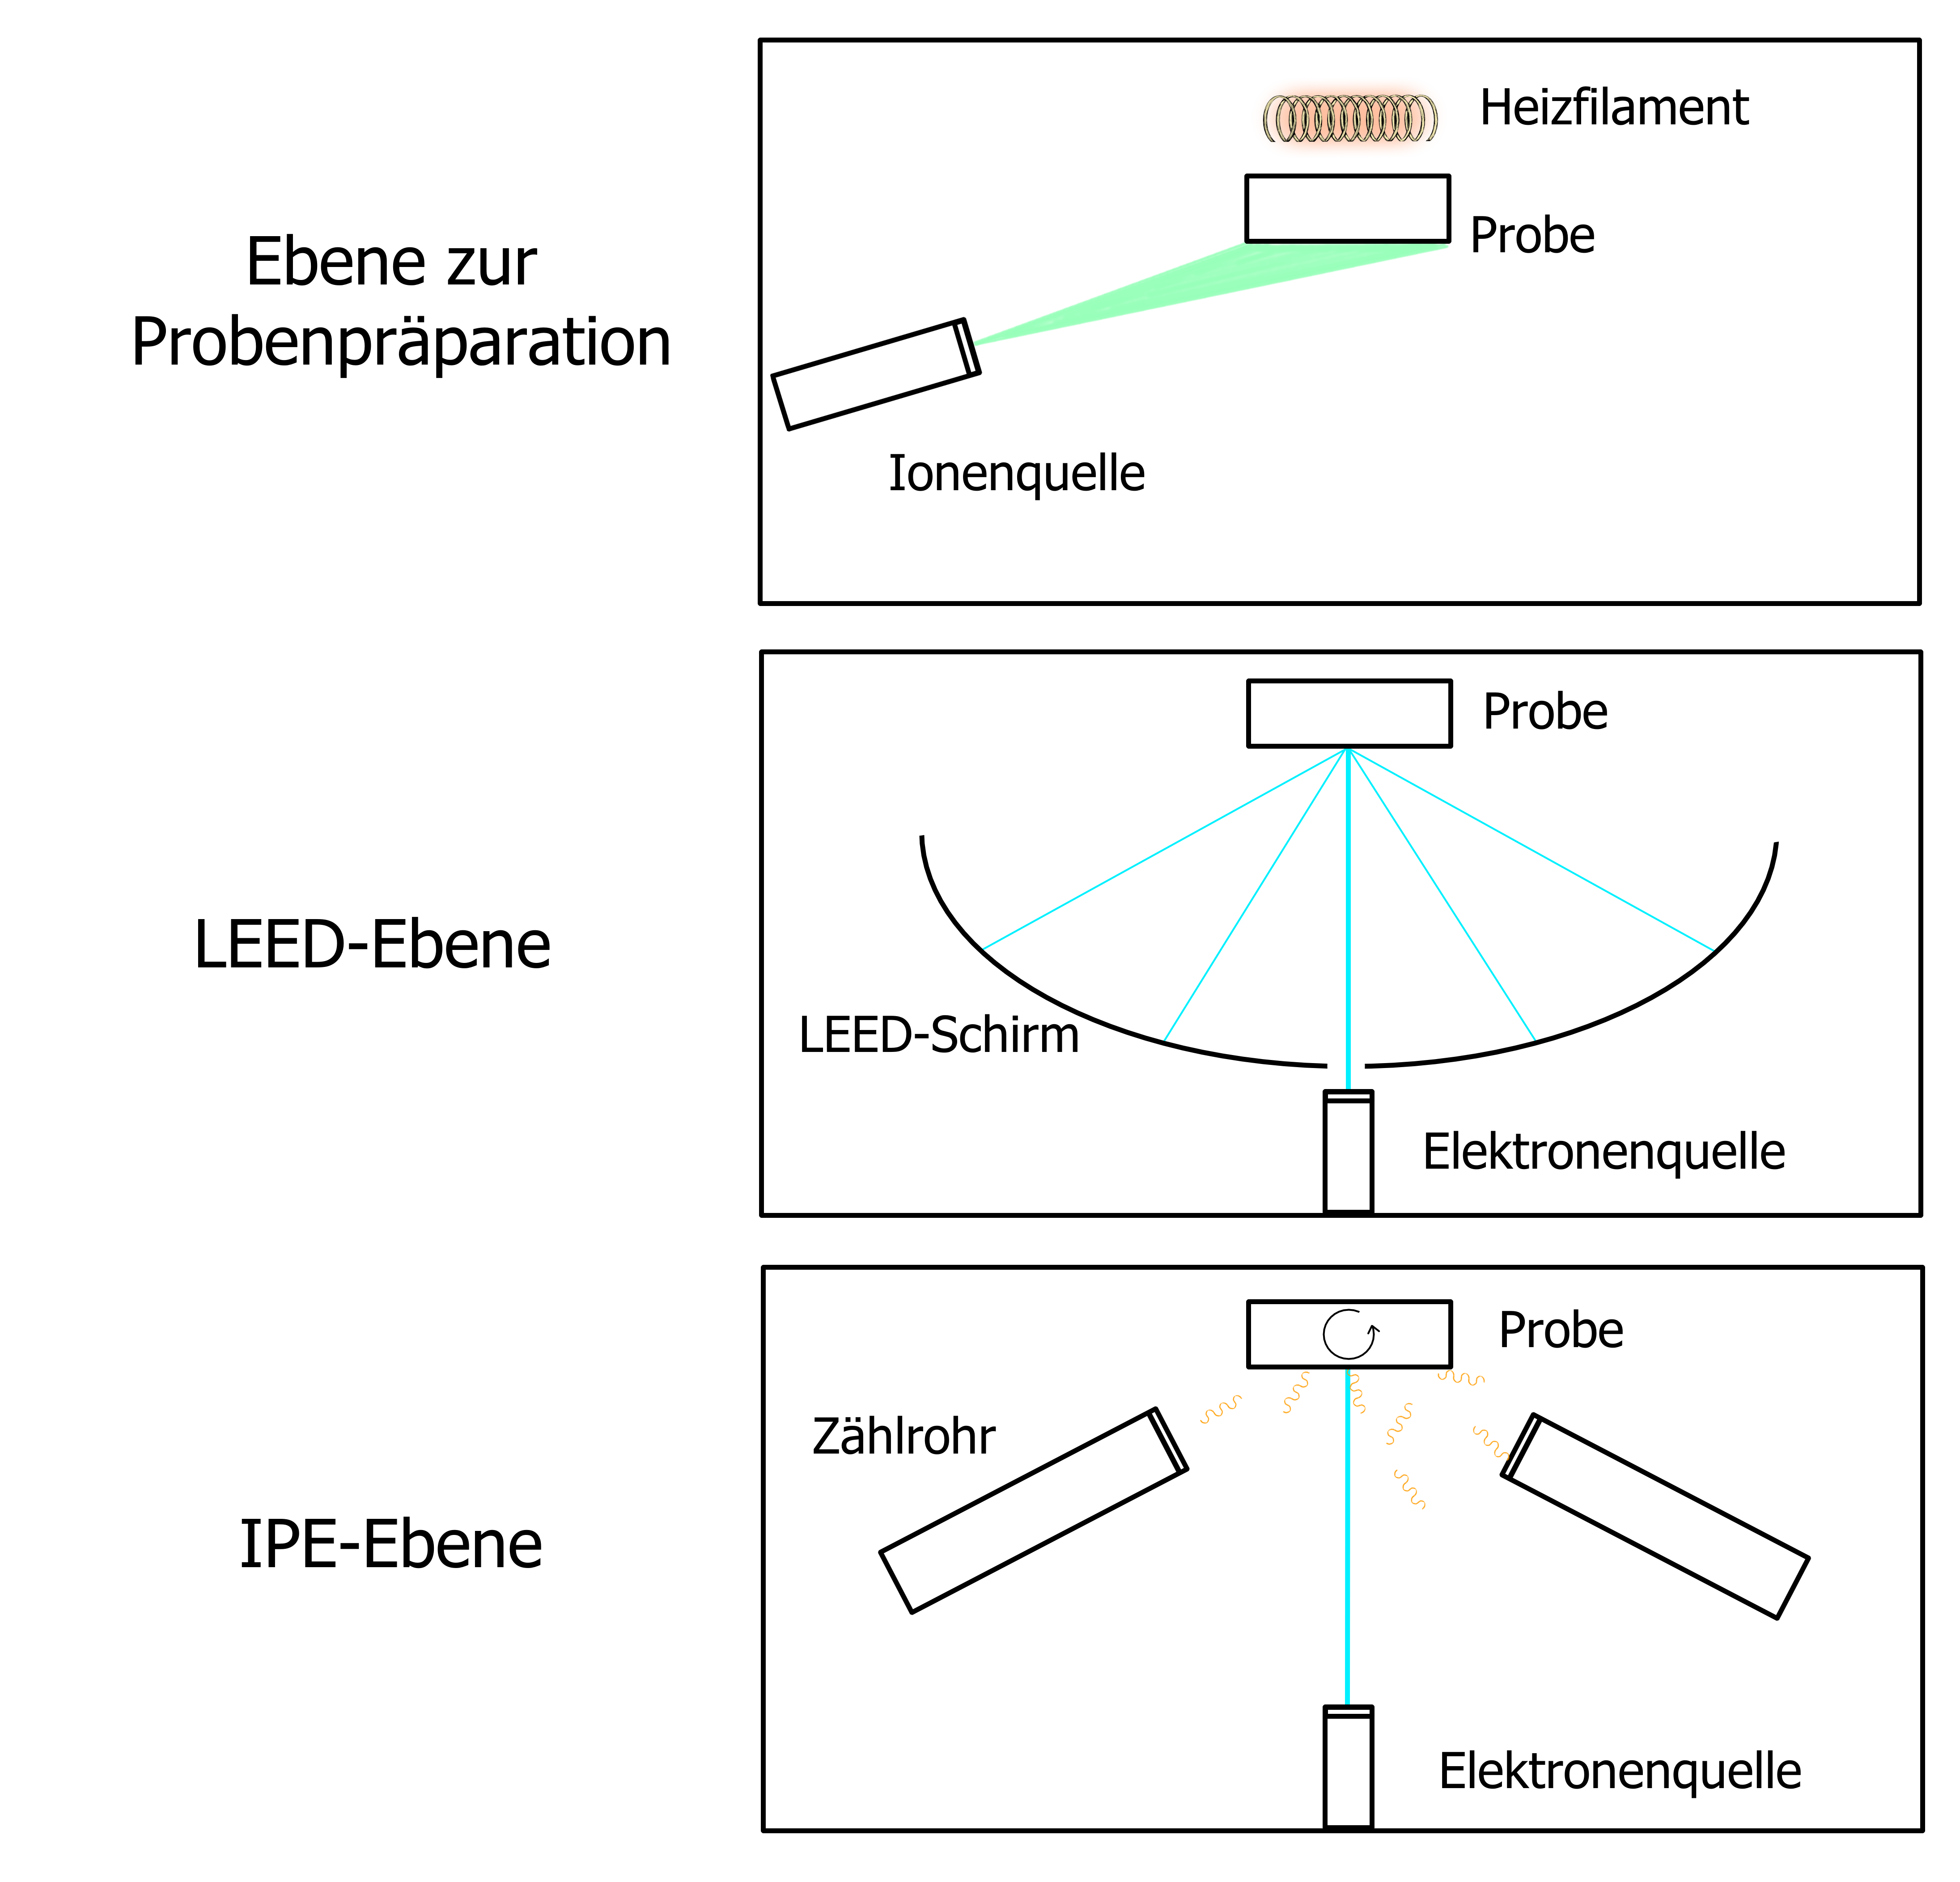
\includegraphics[width=0.75\textwidth]{img/setup1.png}
    \caption{Schematische Darstellung der verschiedenen Ebenen des Versuchaufbaus.
    Nicht dargestellt sind die Vakuumpumpen, der Gaseinlass für die Ionenquelle, der Probeneinlass und der Manipulator über den die Probe zwischen den Ebenen wechseln kann und gekühlt wird.}
    \label{fig_ipe_setup}
\end{figure}
Da alle Anwendungen Hochvakuum benötigen, sind zusätzlich mehrere Vakuumpumpen (Vorpumpe, Turbopumpe) an das Gerät angeschlossen.
Die Probe wird über einen Einlass an dem Manipulator befestigt und kann dann zu den unterschiedlichen Ebenen geschoben werden.
Hier verhalten sich die LEED- und IPE-Ebene wie in \cref{sec:theo1} beschrieben.
Um verschiedene Einstrahlwinkel zu beobachten, werden für die IPE zwei Zählrohre verwendet und es besteht die Möglichkeit die Orientierung der Probenoberfläche über den Manipulator anzupassen.
In der Ebene zur Probenpräparation befinden sich eine Heizspule, um Oberflächenverunreinigungen oder Schutzschichten abzudampfen und eine Ionenquelle zu Sputtern.
Letztere dient dazu glatte Oberflächen herzustellen, weswegen die Einstrahlung nahezu parallel erfolgt.

\subsection{Durchführung \& Diskussion}

Bevor eine IPE-Messung für die $\text{TiSe}_2$-Probe durchgeführt werden kann, ist es notwendig eine Kalibration der Messinstrumente durchzuführen.
Zu diesem Zweck wird ein Kupferkristall verwendet, da er in einer (111)-Orientierung und einem Einstrahlwinkel von \SI{12}{\degree} einen Oberflächenzustand bei ca. \SI{6}{\electronvolt} besitzt, welcher bei \SI{0}{\degree} verschwindet.
Um die Kalibrationsmessung durchzuführen, ist es zunächst nötig das Kupfer zu präparieren.
Dafür wird es auf dem Manipulator angebracht und in die Präparationsebene gefahren.
Damit nur die Verunreinigungen der Oberfläche entfernt werden, wird die Probe auf ihrer Rückseite über den Manipulator gekühlt, während die Vorderseite über das Heizfilament erhitzt wird.
Nach dem Erhitzen wird die Oberfläche mit Argonionen glatt gesputtert.

\begin{figure}[!ht]
    \centering
    \begin{subfigure}{0.495\textwidth}
        \centering
        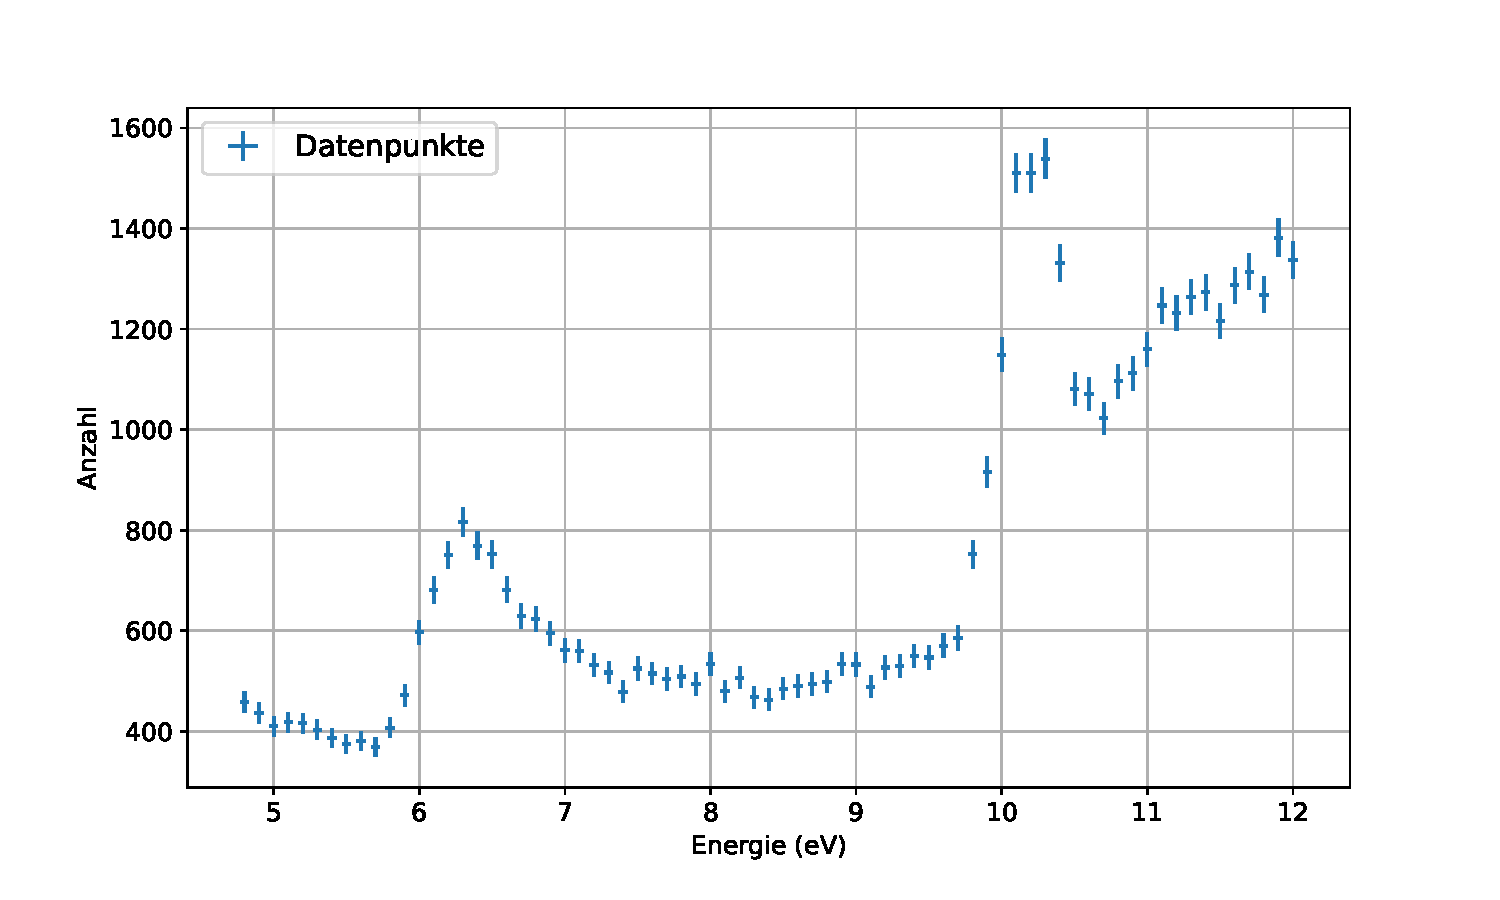
\includegraphics[width=1.1\textwidth]{plots/Cu_0.pdf}
    \caption{}
    \end{subfigure}
    \begin{subfigure}{0.495\textwidth}
        \centering
        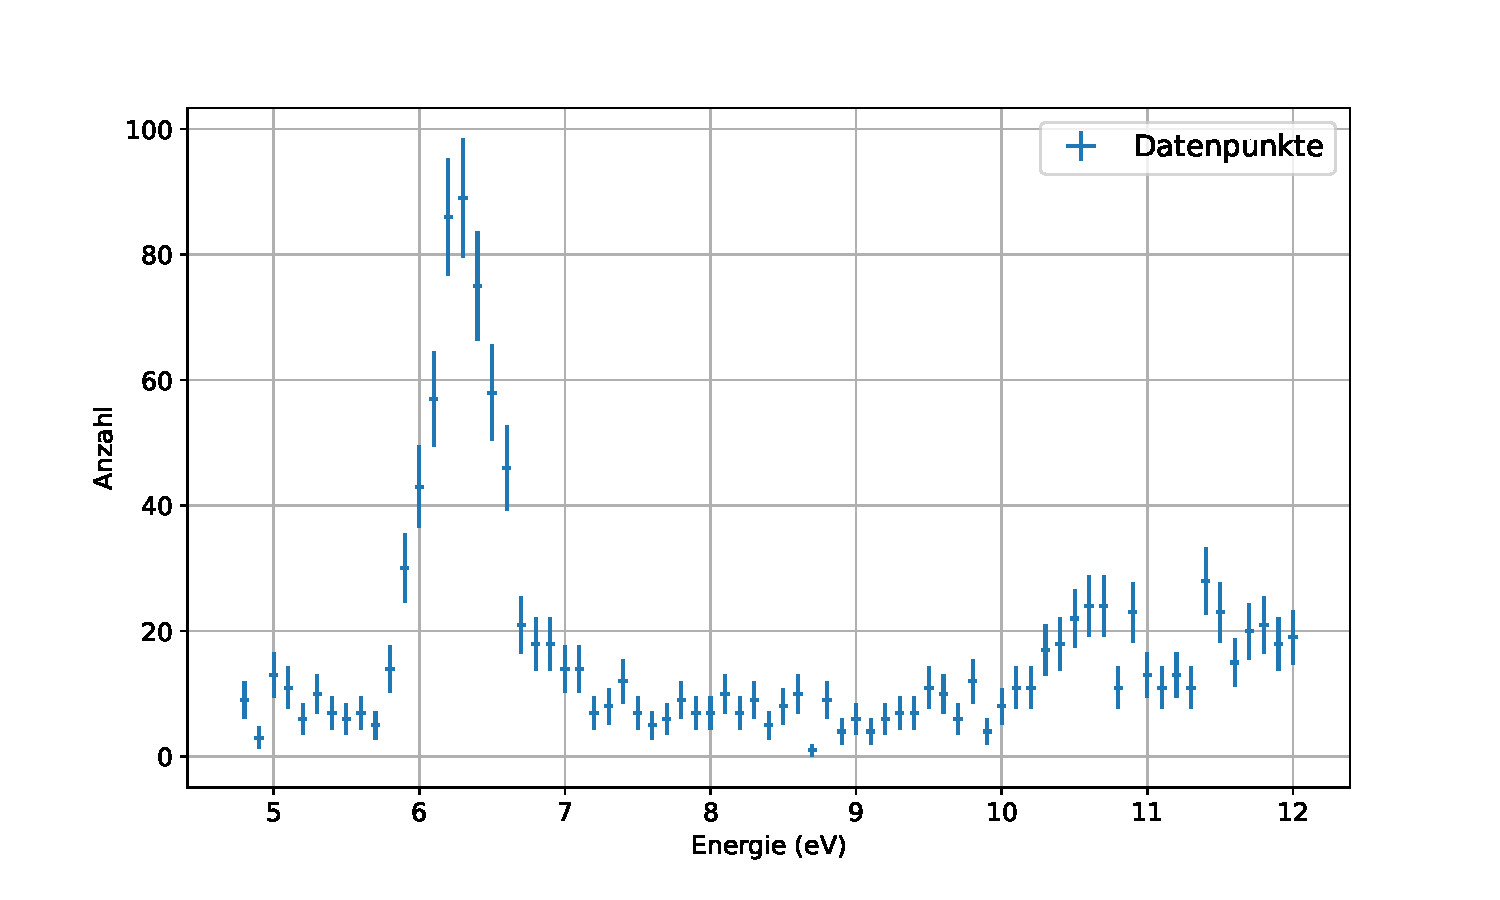
\includegraphics[width=1.1\textwidth]{plots/Cu_12.pdf}
        \caption{}
    \end{subfigure}
    \caption{IPE-Spektren von Kupfer (111) bei (a) \SI{0}{\degree} und (b) \SI{12}{\degree} Einstrahlwinkel.}
    \label{fig_Cu_kal}
\end{figure}
Die daraufhin aufgenommen Kalibrationsspektren für \SI{0}{\degree} und \SI{12}{\degree} sind in \cref{fig_Cu_kal} dargestellt.
Aus dem Verhältnis zum Rauschhintergrund lässt sich der Oberflächenzustand bei \SI{12}{\degree} direkt zu entnehmen.
Da dies bereits nach wenigen Messdurchläufen hervorging, wurden dort deutlich weniger Datenpunkte aufgenommen als bei der \SI{0}{\degree} Messung.
Bei letzterer ist erkennbar, dass der Oberflächenzustand nicht verschwindet, aber ein deutlich kleineres Verhältnis zum Hintergrundrauschen aufweist.
Vermutlich lag keine optimale Probenpräparation vor und es könnten sich über den Messzeitraum Verunreinigungen auf der Probenoberfläche angesammelt haben.
Zur Bestimmung der Unsicherheiten wird $\sqrt{n}$ für die Anzahl $n$ verwendet und für die Energieunsicherheit eine stetige Gleichverteilung über den mittleren Abstand der Datenpunkte.

\

Vor der Messung der $\text{TiSe}_2$-Probe ist jedoch ein weiterer Schritt notwendig, da sich auf der zur Verfügung gestellten Probe eine Schutzschicht aus Selen befindet.
Die Probe wird in der LEED-Ebene betrachtet, wo aufgrund der Selenschicht zusätzliche Beugungsspots erscheinen.
Durch langsames Erhitzen in der Präparationsebene wird die Schutzschicht gelöst und zwischendurch in der LEED-Ebene beobachtet, ob die zusätzlichen Spots noch vorhanden sind.
Sobald sie es nicht mehr sind, wird die Probe unter \SI{200}{\kelvin} auf ca. \SI{190}{\kelvin} gekühlt und die IPE-Messung durchgeführt.
Diese ist \cref{fig_ipe_thighs2} zu sehen.
\begin{figure}[!ht]
    \centering
    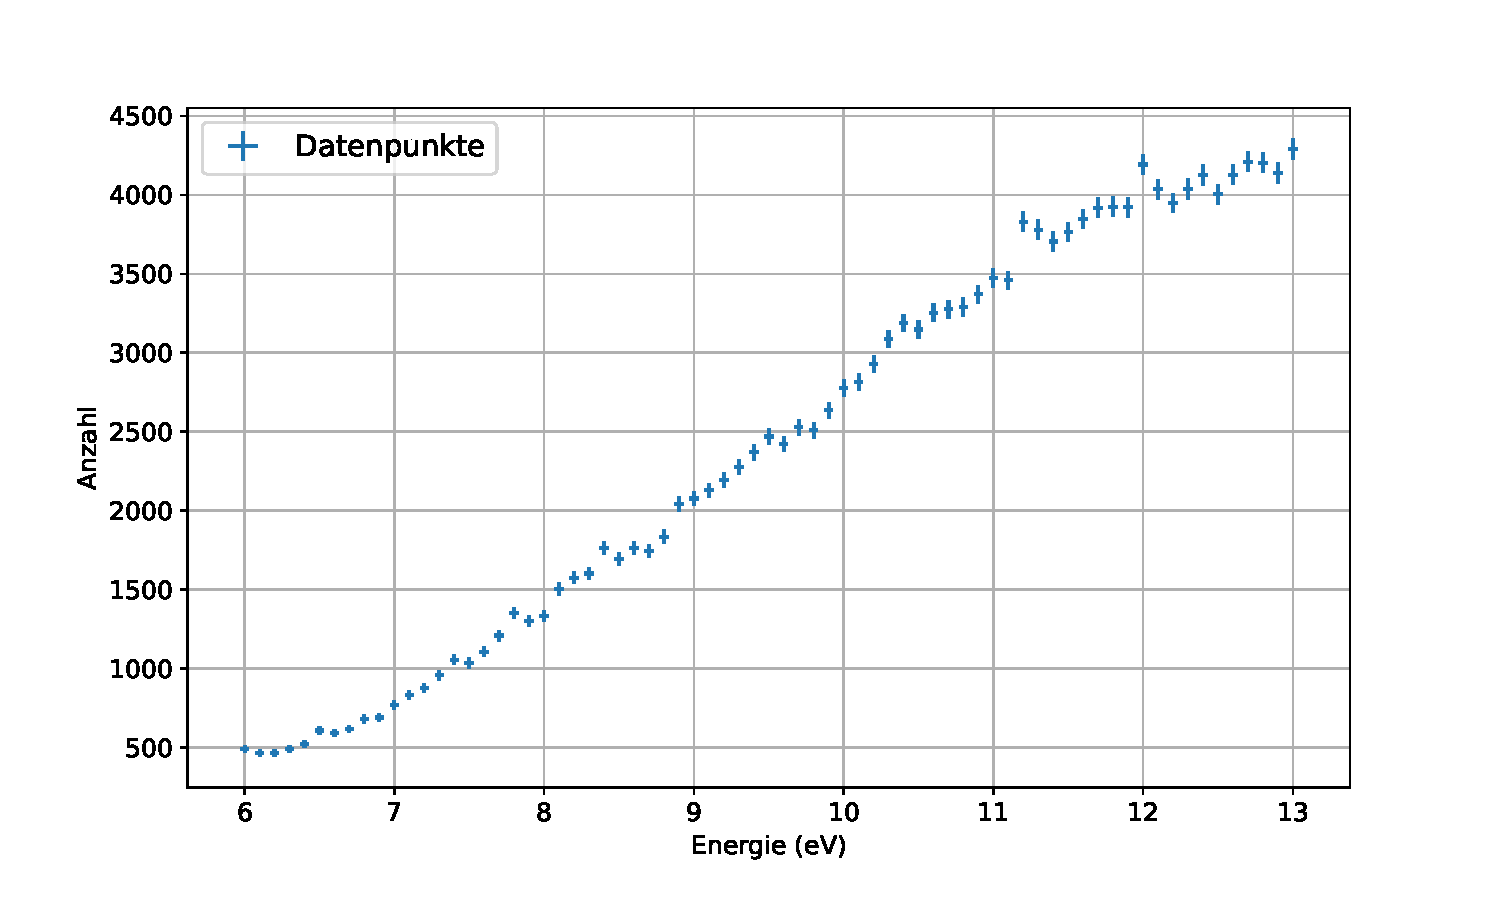
\includegraphics[width=0.85\textwidth]{plots/TiSe2.pdf}
    \caption{IPE-Spektrum der $\text{TiSe}_2$-Probe bei ca. \SI{190}{\kelvin}.}
    \label{fig_ipe_thighs2}
\end{figure}
Hier lässt sich ein annähernd linearer Verlauf erkennen.
Daher ist es unklar, ob sich der gesuchte Zustand im Leitungsband tatsächlich dort befindet.
Der Anstieg liegt vermutlich an IPE von Verunreinigungen, welche sich über die Messzeit auf der Probe abgelagert haben.
Aus den kleineren Peaks bei ca. \SI{11.2}{\electronvolt} oder \SI{12}{\electronvolt} kann aufgrund der geringen Abweichungen vom Hintergrund nichts entnommen werden.

% BroFi Kommentare:

%Warum TiS2? falls das hier war, i dont recall.

%Kupfer 111 OF für Winkelkalibrierung.
%Erst irgendwas sputtern (Argon, iirc). Aceton-Gas für Zählrohr.
%Kühlen für: der manipulator ist ziemlich maissv und da ist kupferblock drin. Wenn der zu warm wird, dampft der krass aus. (500°C für 1h).
%Schnitt senkrecht durch Bandschema. Zwei Messungen, eine nahe Null (Null ja erstmal nicht bekannt) da sollte eigentlich der niederenergetische Zustand verschwinden, weil unter Fermienergie, also nicht zugängig für IPE. Oberer Zustand ist Bildladungszustand.
%Da ist dann noch so zwei Zustände drüber. Die kann man nicht unterscheiden, aber Hoffnung wäre, die zu sehen. (Oder war das schon TiS2? <- ja)

%Zweiter Tag: TiS2 rein. Leed machen. Zwischendurch immer heizen, weil Probe ist mit Selen versiegelt und das will man erst runter haben. Selen ist amorph, also einfach zu erkennen, wie viel davon im leedbild ist.
%Da dann mit warmen (gasförmigen) Stickstoff gekühlt. Oder auch dann mit flüssigem.
%Zwischendurch für die Messung auch immer runterkühlen, weil thermischer Hintergrund
%Dann wieder IPE

	\section{Magnetooptischer Kerr-Effekt}

\subsection{Theoretische Grundlagen}

  \subsubsection{Magnetisierung von Materie}

  Äußere Magnetfelder $\vec{H}$ verusachen in Materie eine materialabhängige makroskopische Magnetisierung $\vec{M}$.
  In dia- ($\chi_V<0$) und paramagnetischen ($\chi_V>0$) Materialien lässt sich dieser Zusammenhang mit der Vakuumpermeabilität $\mu_0$ durch
  \begin{equation}
    \mu_0 \vec{M} = \chi_V \vec{B}_0
  \end{equation}
  beschreiben.
  Die Magnetisierung hängt also über $\chi_V$ linear von der äußeren magnetischen Flussdichte $\vec{B}_0= \mu_0 \vec{H}$ ab.

  In ferromagnetischen Materialien hingegen bleibt nach Abschalten des äußeren Magnetfeldes eine Magnetisierung zurück, die zu der in \cref{fig_magnetismen} abgebildeten Hysteresekurve führt.

  \begin{figure}[H]
      \centering
      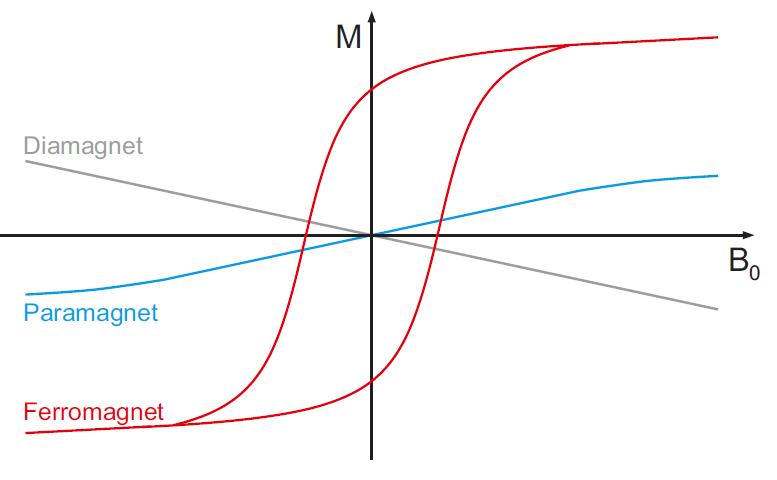
\includegraphics[width=0.7\textwidth]{img/magnetismen}
      \caption{Schematische Abhängigkeit der Magnetisierung $M$ dia-, para- und ferromagnetischer Materialien vom angelegten äußeren Magnetfeld $B$. \cite{anleitung}}
      \label{fig_magnetismen}
  \end{figure}

  %den Kram mit den Domänen lasse ich jetzt weg, weils irgendwie weitgehend egal ist.

  \subsubsection{Polarisation und Materie}
  Die Wechselwirkung von elektromagnetischen Wellen mit Materie kann über den komplexen Brechungsindex
	\begin{align*}
		\tilde{n} = n + ik
	\end{align*}
  mit der Brechung $n$ und der Absorption $k$ beschrieben werden.
  Hieraus kann Reflektion und Transmission berechnet werden.
  Das Hinzufügen eines externen magnetischen Feldes verursacht wie beschrieben eine Magnetisierung in Abhängigkeit von den magnetischen Eigenschaften der Materie.
  Dadurch ändert sich auch der Brechungsindex je nach Polarisation der einfallenden elektromagnetischen Welle.

  Linear polarisiertes Licht kann als Überlagerung einer rechts- und einer linkszirkular polarisierten elektromagnetischen Welle beschrieben werden.
  Beim Treffen auf Materie werden diese Teilwellen mit unterschiedlicher Intensität und Phase reflektiert bzw. transmittiert.
	Im Ergebnis ist die Überlagerung der Wellen nicht mehr linear, sondern elliptisch polarisiert.
	Die Winkeldifferenz zwischen Hauptachse der Ellipse und der Polarisationsrichtung des initialen linear polarisierten Lichts ist die Rotation und die Änderung der Intensität ist die Exzentrizität.

  Die Rotation wird im Falle von Transmission Faraday-Rotation und im Falle von Reflektion Kerr-Rotation mit dem Kerr-Winkel $\theta_K$ genannt.

  In Ferromagneten liegen stets unterschiedlich magnetisierte Domänen (weissche Bezirke) vor.
  Da jedoch bei Messungen des Kerr-Winkels viele Domänen belichtet werden, wird ein mittlerer Kerr-Winkel gemessen, der als proportional zur Magnetisierung angenommen werden kann.

\subsection{Aufbau und Durchführung}

  \begin{figure}[H]
      \centering
      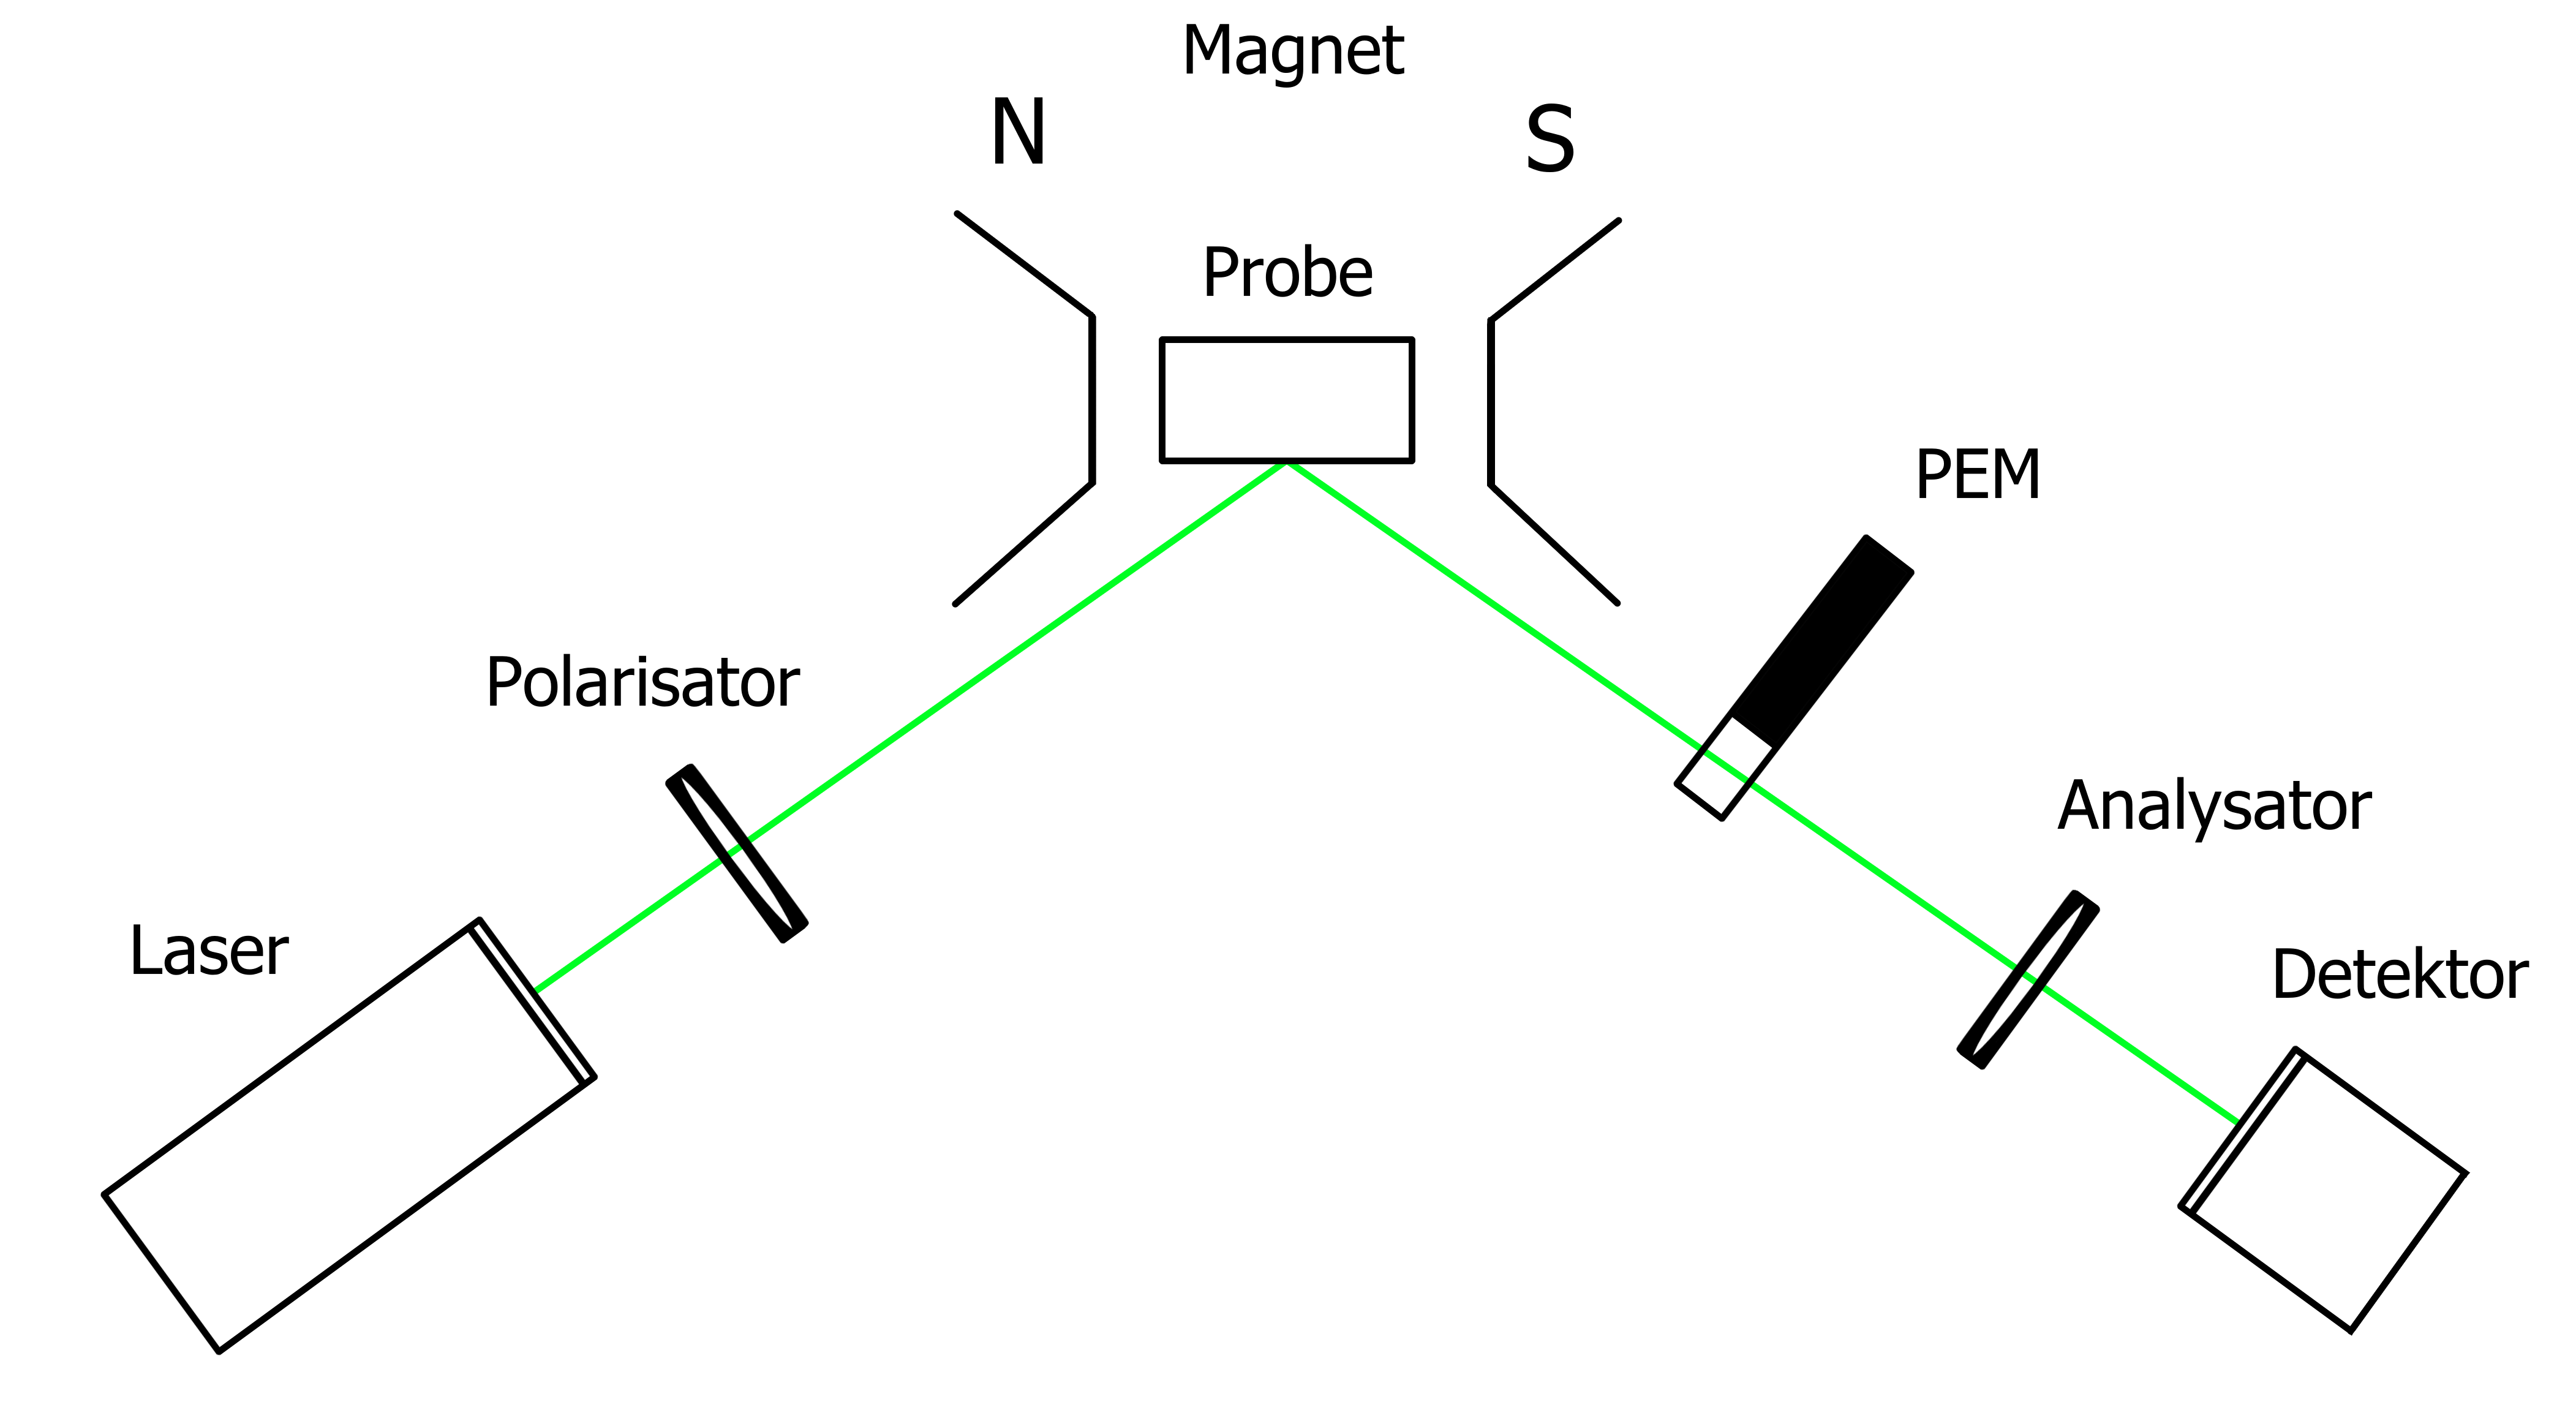
\includegraphics[width=0.8\textwidth]{img/setup2}
      \caption{Schematische Darstellung des experimentellen Aufbaus zur Messung der Magnetisierung in Abhängigkeit vom äußeren Magnetfeld. Abgebildet ist die Konfiguration zur Messung des magnetooptischen Kerr-Effekts in longitudinaler Richtung. Die Polschuhe des Elektromegneten können in der Zeichenebene um \SI{90}{\degree} gedreht werden, um in polarer Richtung messen zu können. PEM steht für photoelastischer Modulator. Die Polarisatoren sind Glan-Thompson-Prismen.}
      \label{fig_setup2}
  \end{figure}

  In \cref{fig_setup2} ist der experimentelle Aufbau dargestellt, der verwendet wird, um die Magnetisierung in Abhängigkeit von einem äußeren Magnetfeld sichtbar zu machen.
  Durch Drehen des Elektromegneten kann die Ausrichtung des Magnetfelds relativ zur Probenebene und Einfallsrichtung geändert werden, sodass in longitudinaler oder polarer Richtung gemessen werden kann.

  Zur Kalibration wird eine Siliziumprobe als Spiegel verwendet, mit dem die optischen Elemente so ausgerichtet werden, dass das gemessene Signal maximiert wird.
  Kupfer ist nicht ferromagnetisch und eignet sich dadurch für die Kalibration.
  Um möglichst empfindlich gegenüber Änderungen der Polarisation zu sein, wird der Analysator in einen \SI{45}{\degree}-Winkel zum Polarisator gebracht, indem der Mittelpunkt zwischen maximaler und minimaler Transmission eingestellt wird.
  Dadurch bewegt sich die Polarisation auf der Flanke der $\cos ^2$-Kurve des Gesetzes von Malus, sodass kleine Änderungen in der Polarisation zu einer maximalen Änderung der Intensität führen.
  Außerdem kann die Kurve in der Nähe dieses Punktes als linear genähert werden, sodass eine Proportionalität zwischen Intensitätsänderung und Polarisationsänderung besteht.

  Dann wird eine Kalibrationsmessung für das Magnetfeld durchgeführt, indem eine Hall-Sonde an die Stelle der Probe gebracht wird und der Spulenstrom schrittweise erhöht wird.
  Es wird ein photoelastischer Modulator verwendet, um dem reflektierten Laserstrahl eine Modulation hinzuzufügen, die in Kombination mit einem Lock-In-Verstärker eine erhöhte Messgenauigkeit erlaubt.
  Da lediglich über die Intensität auf den Kerr-Winkel und über diesen auf die Magnetisierung geschlossen wird, ist es nur möglich, die Magnetisierung in willkürlichen Einheiten anzugeben.

  Es werden je zehn Messkurven für eine CoPt-Probe und eine CrO$_2$-Probe aufgenommen, indem der Spulenstrom graduell erhöht und wieder gesenkt wird, sodass die Hysteresekurve gemessen wird.
  Sollte sich schnell herausstellen, dass die Magnetisierbarkeit der Probe in einer Magnetfeldausrichtung nicht messbar ist, wird keine vollständige Messung durchgeführt. %er meinte, in der Richtung nicht magnetisierbar. Das hieße ja, dass das Einkristalle sind. Man könnte halt auch behaupten, dass einfach in der Richtung kein moke, aber trotzdem Magnetisierung stattfindet.


\subsection{Ergebnisse und Diskussion}

%CoPt ist nur Out of plane Magnetisierbar. Der CrO2 nur in plane. Die jeweils anderen nur kurz gemessen, um das festzustellen.
CoPt ist nur in der polaren Messung magnetisierbar und CrO$_2$ nur in der longitudinalen Messung.
Die Unsicherheit der Magnetisierung wird auf Basis der Streuung der Daten bei im Betrag hohen Magnetfeldstärken abgeschätzt, da hier die Magnetisierung konstant sein sollte.
Die Unsicherheit der Magnetfeldstärke wird als demgegenüber vernachlässigbar angenommen.

\begin{figure}[H]
    \centering
    \begin{subfigure}{0.465\textwidth}
        \centering
        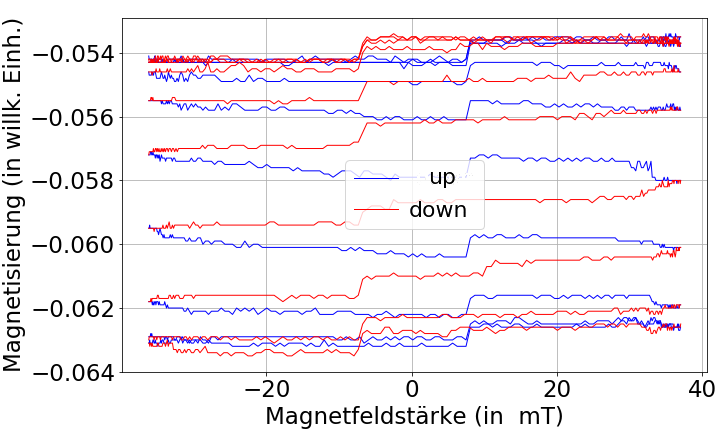
\includegraphics[width=1.1\textwidth]{plots/swp_cro_raw}
    \caption{CrO$_2$}
    \end{subfigure}
    \hfill
    \begin{subfigure}{0.465\textwidth}
        \centering
        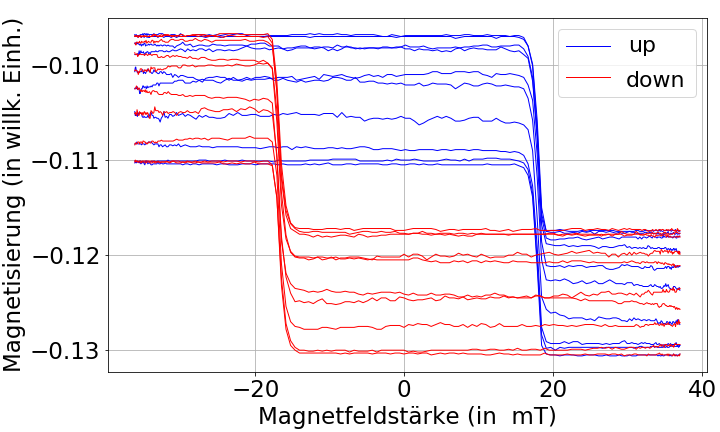
\includegraphics[width=1.1\textwidth]{plots/swp_copt_raw}
        \caption{CoPt}
    \end{subfigure}
    \caption{Unbearbeitete Messdaten beider Proben. \enquote{up} steht für steigende und \enquote{down} für fallende Magnetfeldstärke. Die Unsicherheiten wurden zugunsten der Übersicht nicht dargestellt.}
      \label{fig_moke_raw}
\end{figure}

  In \cref{fig_moke_raw} ist das Ergebnis der Messungen dargestellt.
  Es ist deutlich sichtbar, dass während der Messung ein thermischer Drift stattfindet, der die gemessene Intensität über die Messungen wandern lässt.
  Da die Remanenz der CrO$_2$-Probe deutlich kleiner ist, fällt dies hier stärker ins Gewicht.
  Um dies zu korrigieren werden zunächst alle Messungen über ihren Mittelwert so angepasst, dass die durchschnittliche Intensität der Messungen (für auf- und absteigende Messungen einzeln) etwa konstant ist.
  Zusätzlich wird ein konstanter thermischer Drift innerhalb der Messungen angenommen und die Messungen so korrigiert, dass die Kurven bei im Betrag sehr hohen Magnetfeldern konstant sind.
  Dies ist in \cref{fig_moke_einzeln} abgebildet.
  Hier wird auch sichtbar, dass die geringe Präzision der Gleitkommazahlen im Messergebnis bei der CrO$_2$-Probe aufgrund der geringen Remanenz zu Rundungsfehlern führt. %Genius...

\begin{figure}[H]
    \centering
    \begin{subfigure}{0.495\textwidth}
        \centering
        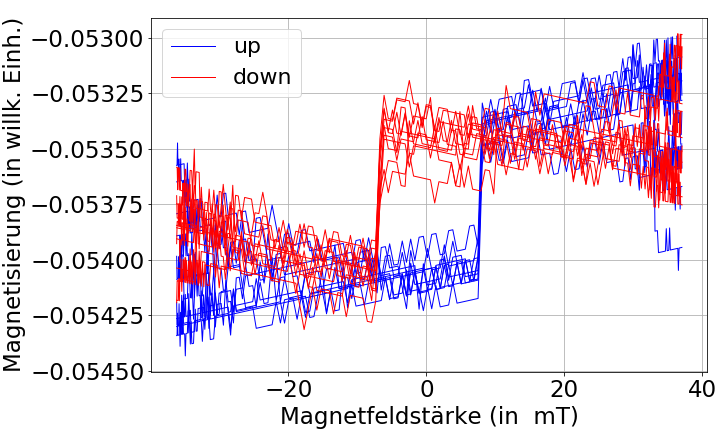
\includegraphics[width=1.1\textwidth]{plots/swp_all_magn_cro}
    \caption{CrO$_2$}
    \end{subfigure}
    \begin{subfigure}{0.495\textwidth}
        \centering
        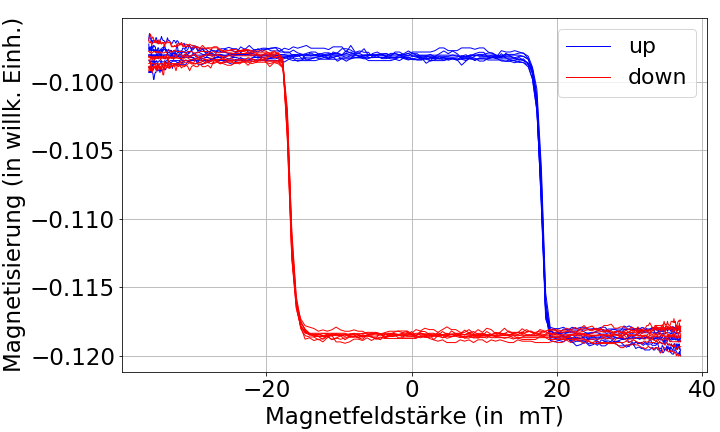
\includegraphics[width=1.1\textwidth]{plots/swp_all_magn_copt}
        \caption{CoPt}
    \end{subfigure}
    \caption{Um den thermischen Drift korrigierte Messungen der Hysteresekurven von CrO$_2$ und CoPt. \enquote{up} steht für steigende und \enquote{down} für fallende Magnetfeldstärke. Die Unsicherheiten wurden zugunsten der Übersicht nicht dargestellt.}
    \label{fig_moke_einzeln}
\end{figure}



\begin{figure}[H]
    \centering
    \begin{subfigure}{0.495\textwidth}
        \centering
        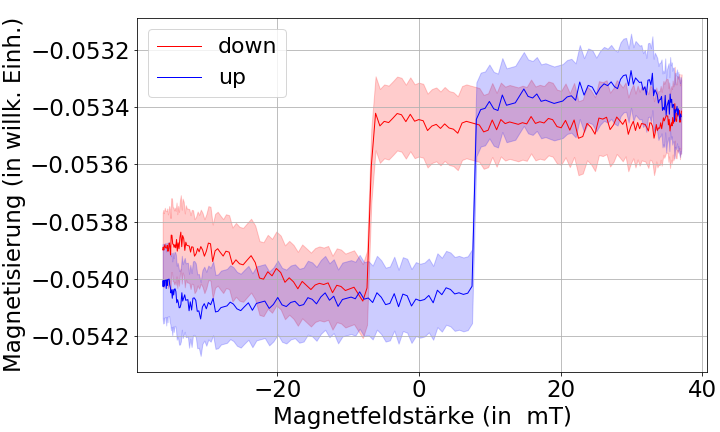
\includegraphics[width=1.1\textwidth]{plots/swp_avg_magn_man_cro}
    \caption{CrO$_2$}
    \end{subfigure}
    \begin{subfigure}{0.495\textwidth}
        \centering
        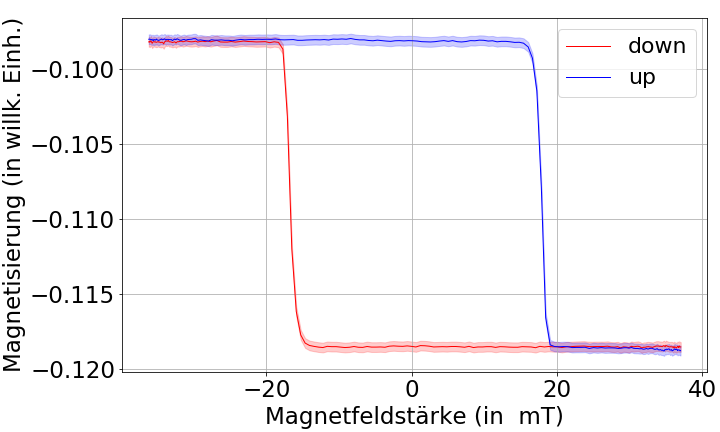
\includegraphics[width=1.1\textwidth]{plots/swp_avg_magn_man_copt}
        \caption{CoPt}
    \end{subfigure}
    \caption{Gegen den thermischen Drift korrigierte gemittelte Messungen der Hysteresekurven von CrO$_2$ und CoPt. \enquote{up} steht für steigende und \enquote{down} für fallende Magnetfeldstärke.}
    \label{fig_moke_averages}
\end{figure}

Aus diesen zehn Messungen werden nun jeweils Mittelwerte gebildet und in \cref{fig_moke_averages} dargestellt.
Es ist bei beiden Messungen deutlich die Hysterese zu erkennen, wobei im Falle der CoPt-Probe die Koerzitivfeldstärke und Remanenz deutlich höher sind (siehe \cref{tab:remko}).

\begin{table}[H]
	\centering
	\caption{Gemessene Remanenz und Koerzitivfeldstärke beider Proben, Remanenz in willkürlichen Einheiten.}
	\begin{tabular}{c| c | c}
		Probe & Remanenz & Koerzitivfeldstärke \\ \hline
    CrO$_2$ & \SI{0,000315+-0,00018}{} & \SI{14,74+-0,45}{mT} \\
    CoPt & \SI{0,01015+-0,0005}{}  & \SI{34,6+-0,6}{mT} \\
	\end{tabular}
	\label{tab:remko}
\end{table}

	\newpage
\section{Schlussfolgerung}
	% Rückgriff auf Hypothese und drittes Nennen dieser
	% Quellen zitieren, Websiten mit Zugriffsdatum
	% Verweise auf das Laborbuch (sind erlaubt)
	% Tabelle + Bilder mit Beschriftung
	%TODO schauen, ob hier was angepasst werden muss,

	Insgesamt lässt sich sagen, dass die verschiedenen Teilversuche erfolgreich durchgeführt werden konnten.
	Mit dem SEM konnte eine Auflösung von unter \SI{300}{nm} erreicht werden und anhand von EDX-Messungen Elementkonzentrationen in einer Messingprobe und Elementverteilungen in einer geteilten Probe bestimmt werden.
	Womöglich könnte im SEM eine bessere Auflösung durch Optimierung des Strahlengangs erreicht werden.
	Dies könnte beispielsweise durch Anpassung des Linsensystems und der Aberrationskorrekturen erreicht werden.
	Der damit verbundene Zeitaufwand hätte jedoch den Rahmen dieser Untersuchung überstiegen.

	Im TEM konnte eine Auflösung erreicht werden, die die Bestimmung der Abstände von Atomebenen ermöglicht.
	Diese wurden sowohl im Realraumbild als auch im Bild in der Streuebene bestimmt.

	Zuletzt wird das EEL-Spektrum der Probe aufgenommen und Plasmonen- und Selen-Peaks identifiziert.

		% --- Anhang einbinden
	\newpage
\appendix
\section{Appendix}\label{sec:appendix}

\subsection{Uncertainties}\label{sec:uncertainties}

Any uncertainties will be calculated in accordance with GUM.
The equations used for that are seen in (\ref{fig:GUM_combine}) and (\ref{fig:GUM_formula}).
For the calculations the python library "uncertainties" will be used, which follows the guidelines of GUM.
As for the uncertainties of specific parameters the approximation curves of the $y$-uncertainties of those parameters will be regarded and the method of least squares used.
Here the method "scipy.optimize.curve\_fit()" from the uncertainties library is taken.

\begin{figure}[ht]
	\begin{equation*}
	x = \sum_{i=1}^{N} x_i
	;\quad
	\sigma_x = \sqrt{\sum_{i = 1}^{N} \sigma_{x_i}^2}
	\end{equation*}
	\caption{Formel für kombinierte Unsicherheiten des selben Typs nach GUM.}
	\label{fig:GUM_combine}
\end{figure}

\begin{figure}[ht]
	\begin{align*}
	f = f(x_1, \dots , x_N)
	;\quad
	\sigma_f = \sqrt{\sum_{i = 1}^{N}\left(\pdv{f}{x_i} \sigma_{x_i}\right) ^2}
	\end{align*}
	\caption{Formel für sich fortpflanzende Unsicherheiten erster Ordnung nach GUM.}
	\label{fig:GUM_formula}
\end{figure}

%\newpage
%\subsection{weitere Abbildungen}

\newpage
\subsection{SPEs additional figures}
\label{sec:anhang:spe}

\begin{figure}[H]
    \centering
    \begin{subfigure}{0.47\textwidth}
        \centering
        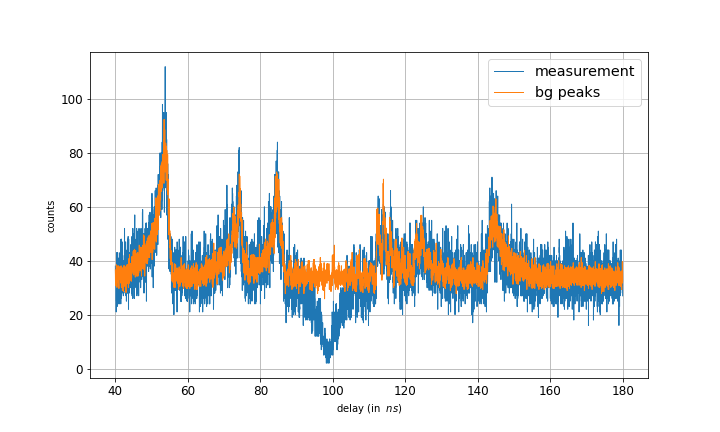
\includegraphics[width=1.0\textwidth]{img/output_t2/50.0muW_bg_peaks.png}
    		\caption{}
    		%\label{fig_antibunch_background_comp}
    \end{subfigure}
    %\hfill
    \begin{subfigure}{0.47\textwidth}
        \centering
        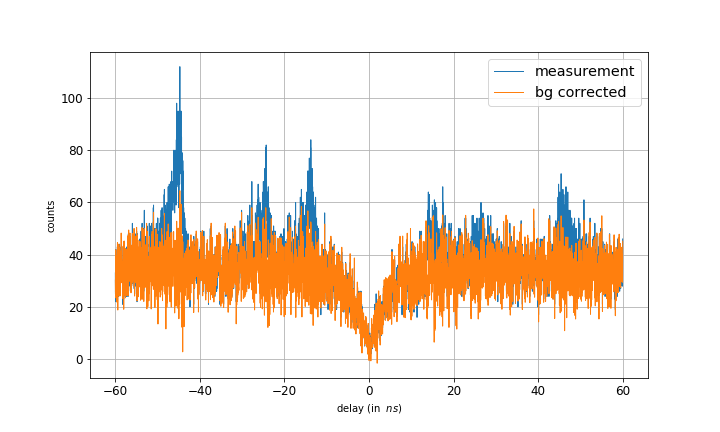
\includegraphics[width=\textwidth]{img/output_t2/50.0muW_bg_vgl.png}
        \caption{}
        %\label{fig_antibunch_raw_corr_comp}
    \end{subfigure}
    \caption{a: Antibunching measurement as recorded and compared to the adjusted background signal. b: Antibunching measurement as recorded and compared to the background corrected signal. The laser power is \SI{50}{\micro W}.} %hoffe ok, dass der eine so doppelt ist
	%\label{fig_antibunch_comp}
\end{figure}
\begin{figure}[H]
    \centering
    \begin{subfigure}{0.47\textwidth}
        \centering
        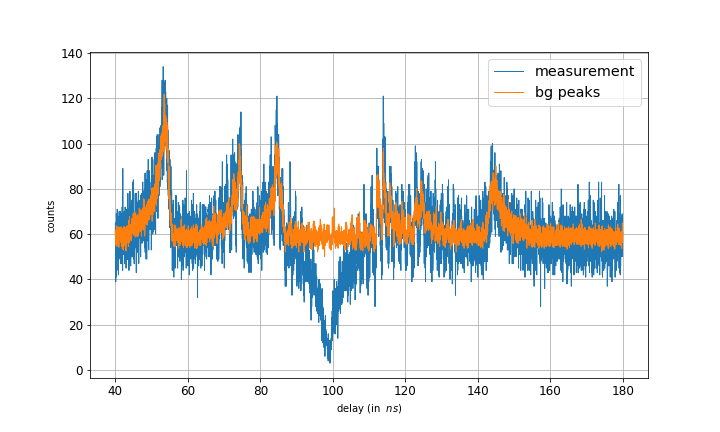
\includegraphics[width=1.0\textwidth]{img/output_t2/100.0muW_bg_peaks.png}
    \caption{}
    %label{fig_antibunch_background_comp}
    \end{subfigure}
    %\hfill
    \begin{subfigure}{0.47\textwidth}
        \centering
        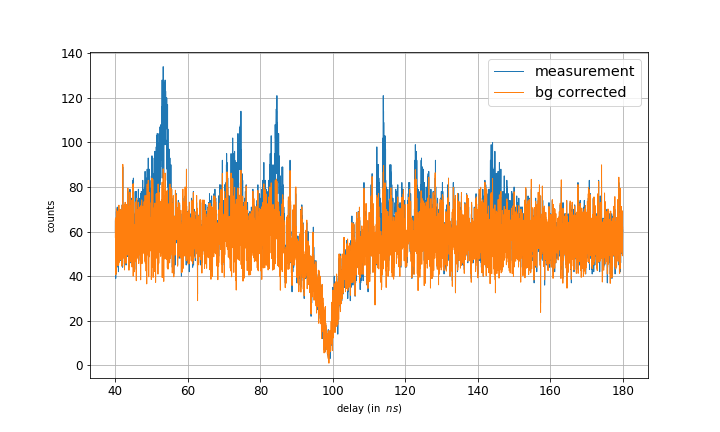
\includegraphics[width=\textwidth]{img/output_t2/100.0muW_bg_vgl.png}
        \caption{}
        %label{fig_antibunch_raw_corr_comp}
    \end{subfigure}
    \caption{a: Antibunching measurement as recorded and compared to the adjusted background signal. b: Antibunching measurement as recorded and compared to the background corrected signal. The laser power is \SI{100}{\micro W}.} %hoffe ok, dass der eine so doppelt ist
	%label{fig_antibunch_comp}
\end{figure}
\begin{figure}[H]
    \centering
    \begin{subfigure}{0.47\textwidth}
        \centering
        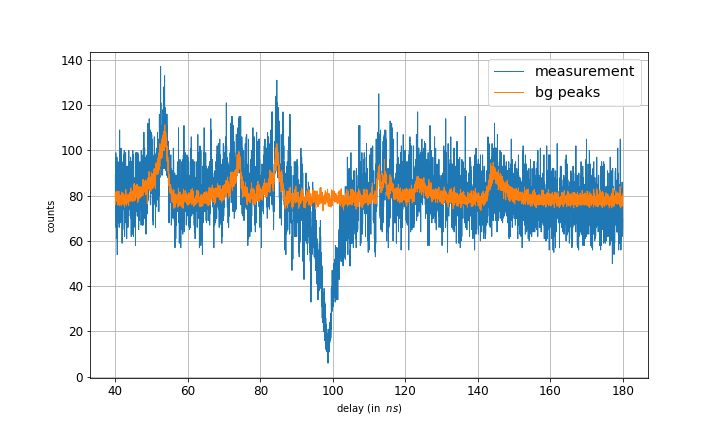
\includegraphics[width=1.0\textwidth]{img/output_t2/250.0muW_bg_peaks.png}
    \caption{}
    %label{fig_antibunch_background_comp}
    \end{subfigure}
    %\hfill
    \begin{subfigure}{0.47\textwidth}
        \centering
        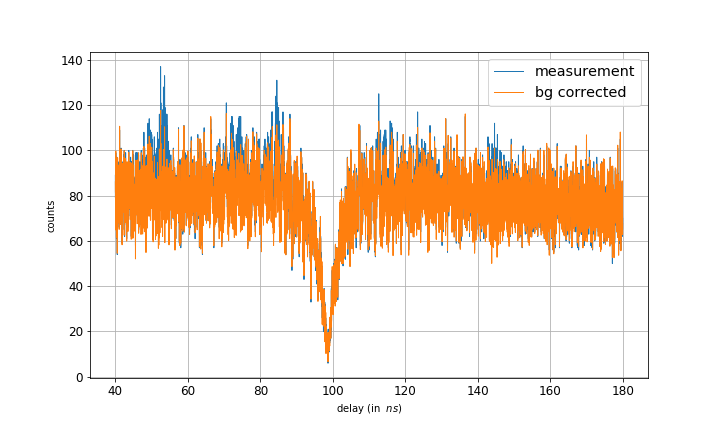
\includegraphics[width=\textwidth]{img/output_t2/250.0muW_bg_vgl.png}
        \caption{}
        %label{fig_antibunch_raw_corr_comp}
    \end{subfigure}
    \caption{a: Antibunching measurement as recorded and compared to the adjusted background signal. b: Antibunching measurement as recorded and compared to the background corrected signal. The laser power is \SI{250}{\micro W}.} %hoffe ok, dass der eine so doppelt ist
	%label{fig_antibunch_comp}
\end{figure}
\begin{figure}[H]
    \centering
    \begin{subfigure}{0.47\textwidth}
        \centering
        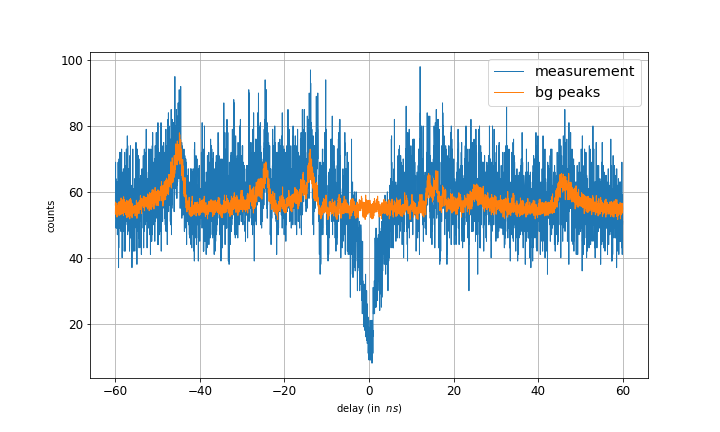
\includegraphics[width=1.0\textwidth]{img/output_t2/500.0muW_bg_peaks.png}
    \caption{}
    %label{fig_antibunch_background_comp}
    \end{subfigure}
    %\hfill
    \begin{subfigure}{0.47\textwidth}
        \centering
        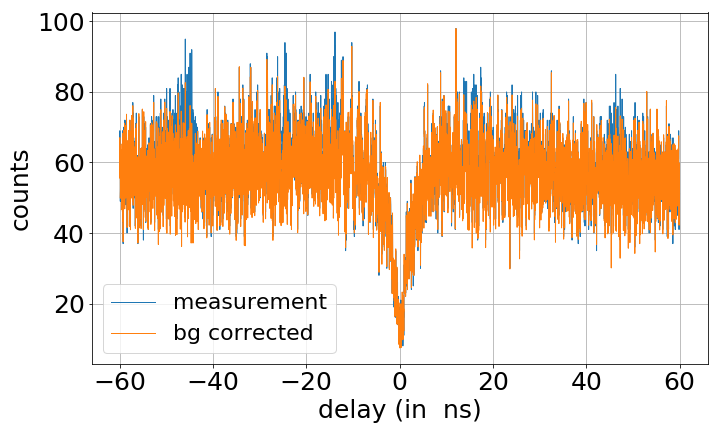
\includegraphics[width=\textwidth]{img/output_t2/500.0muW_bg_vgl.png}
        \caption{}
        %label{fig_antibunch_raw_corr_comp}
    \end{subfigure}
    \caption{a: Antibunching measurement as recorded and compared to the adjusted background signal. b: Antibunching measurement as recorded and compared to the background corrected signal. The laser power is \SI{500}{\micro W}.} %hoffe ok, dass der eine so doppelt ist
	%label{fig_antibunch_comp}
\end{figure}
\begin{figure}[H]
    \centering
    \begin{subfigure}{0.47\textwidth}
        \centering
        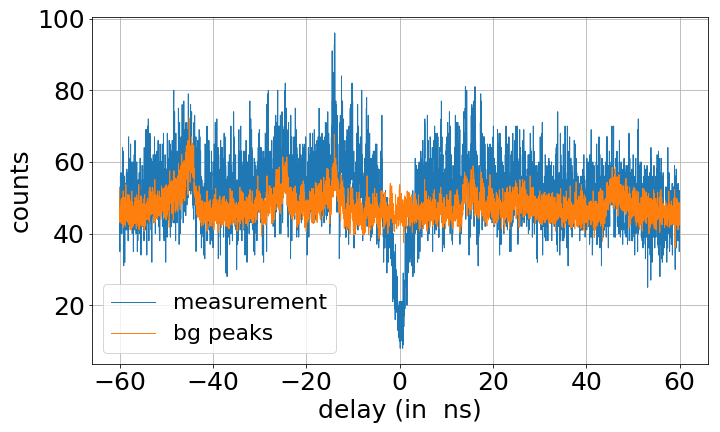
\includegraphics[width=1.0\textwidth]{img/output_t2/1000.0muW_bg_peaks.png}
    \caption{}
    %label{fig_antibunch_background_comp}
    \end{subfigure}
    %\hfill
    \begin{subfigure}{0.47\textwidth}
        \centering
        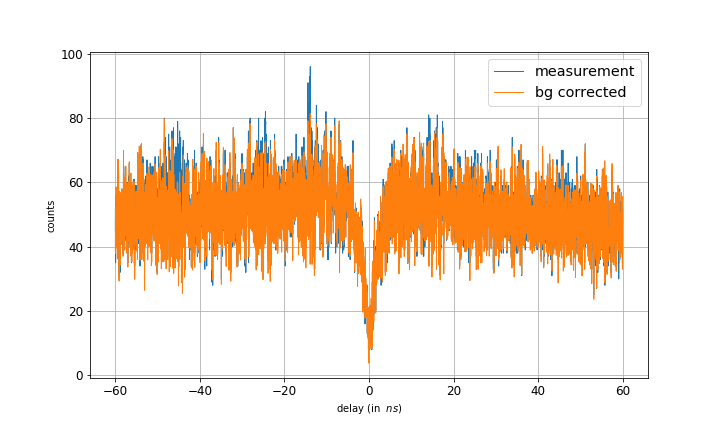
\includegraphics[width=\textwidth]{img/output_t2/1000.0muW_bg_vgl.png}
        \caption{}
        %label{fig_antibunch_raw_corr_comp}
    \end{subfigure}
    \caption{a: Antibunching measurement as recorded and compared to the adjusted background signal. b: Antibunching measurement as recorded and compared to the background corrected signal. The laser power is \SI{1000}{\micro W}.} %hoffe ok, dass der eine so doppelt ist
	%label{fig_antibunch_comp}
\end{figure}
\begin{figure}[H]
    \centering
    \begin{subfigure}{0.47\textwidth}
        \centering
        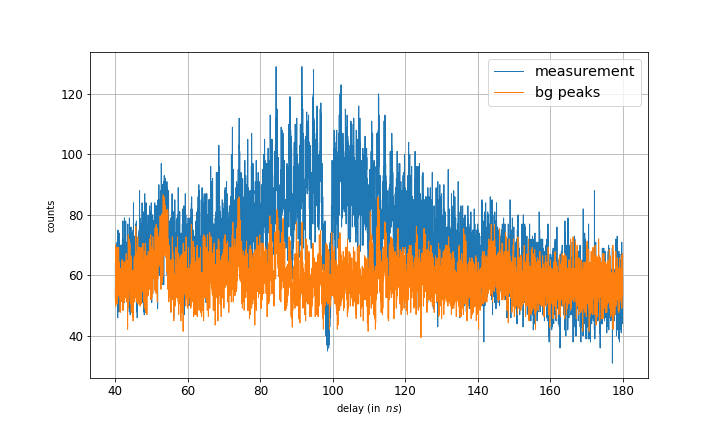
\includegraphics[width=1.0\textwidth]{img/output_t2/2000.0muW_bg_peaks.png}
    \caption{}
    %label{fig_antibunch_background_comp}
    \end{subfigure}
    %\hfill
    \begin{subfigure}{0.47\textwidth}
        \centering
        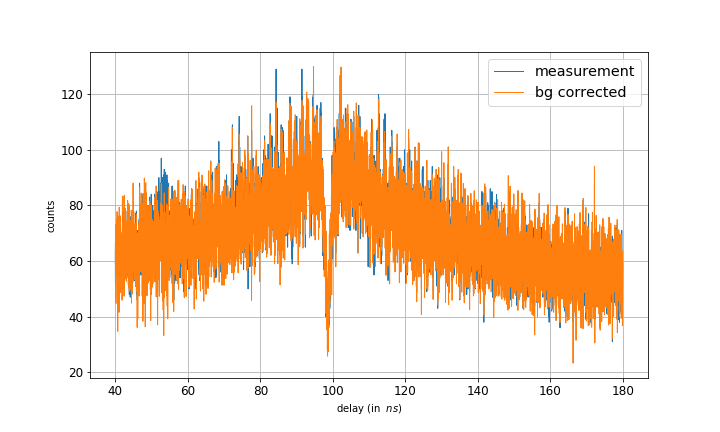
\includegraphics[width=\textwidth]{img/output_t2/2000.0muW_bg_vgl.png}
        \caption{}
        %label{fig_antibunch_raw_corr_comp}
    \end{subfigure}
    \caption{a: Antibunching measurement as recorded and compared to the adjusted background signal. b: Antibunching measurement as recorded and compared to the background corrected signal. The laser power is \SI{2000}{\micro W}.} %hoffe ok, dass der eine so doppelt ist
	%label{fig_antibunch_comp}
\end{figure}

\newpage
\subsection{Faraday Rotation additional figures}
\label{sec:anhang:far}

\begin{figure}[H]
    \centering
    \begin{subfigure}{0.47\textwidth}
        \centering
        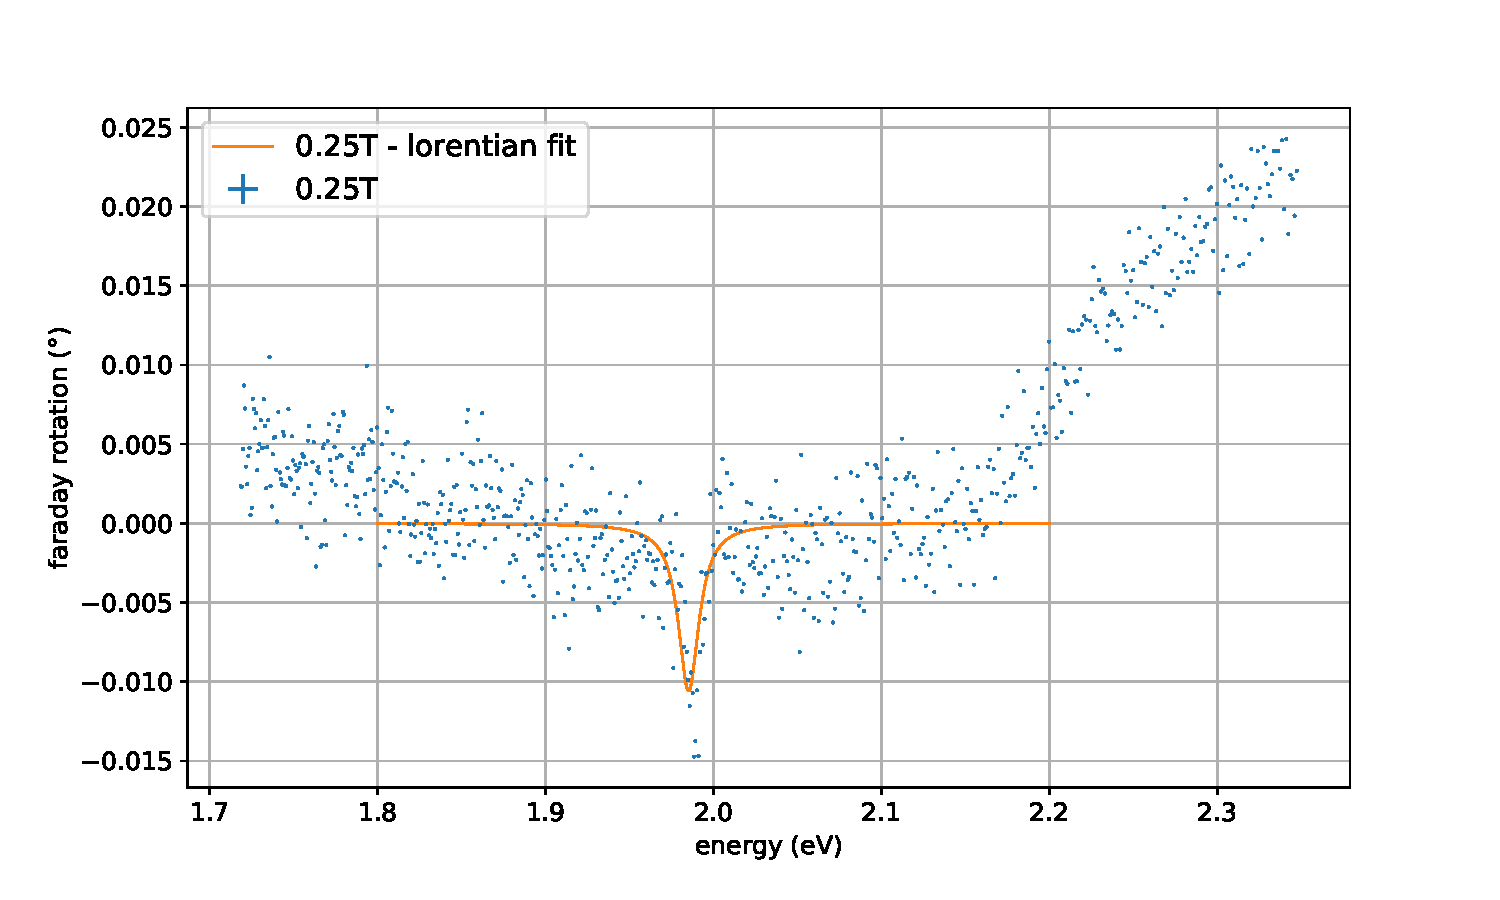
\includegraphics[width=1.0\textwidth]{plots/WS2_250mT.pdf}
    \caption{}
    %label{fig_antibunch_background_comp}
    \end{subfigure}
    %\hfill
    \begin{subfigure}{0.47\textwidth}
        \centering
        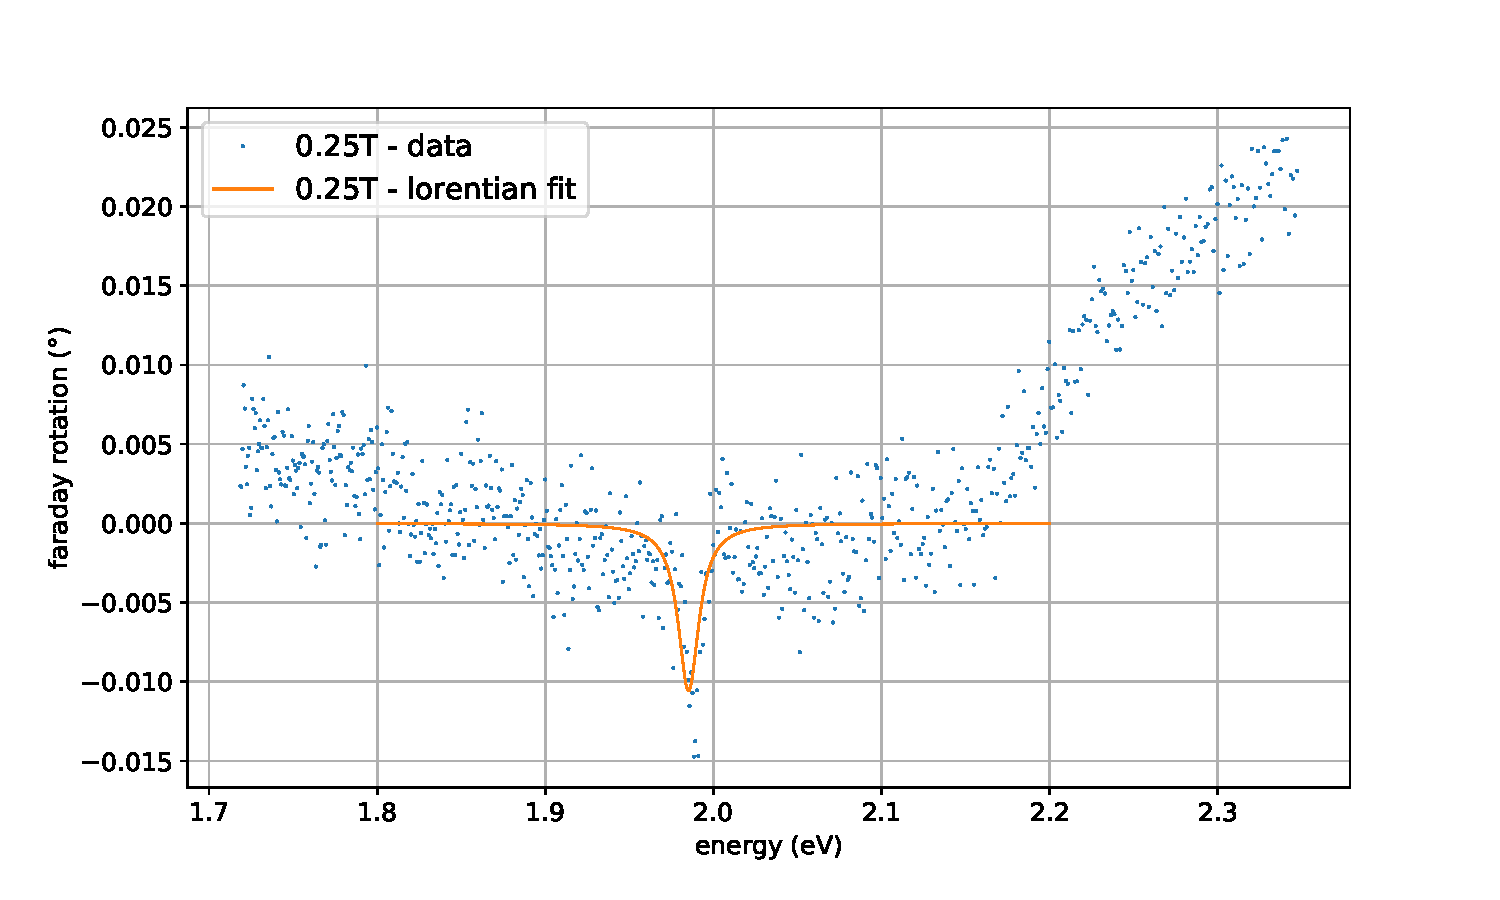
\includegraphics[width=\textwidth]{plots/WS2_250mT_noerror.pdf}
        \caption{}
        \label{fig_WS2_250mT_noerror}
    \end{subfigure}
    \caption{a: Representation of WS$_2$ monolayer data points of the faraday rotation with external magnetic field of \SI{0.25}{\tesla} and lorentian fit. b: Same as a, but without errorbars.} %hoffe ok, dass der eine so doppelt ist
\end{figure}

\begin{figure}[H]
    \centering
    \begin{subfigure}{0.47\textwidth}
        \centering
        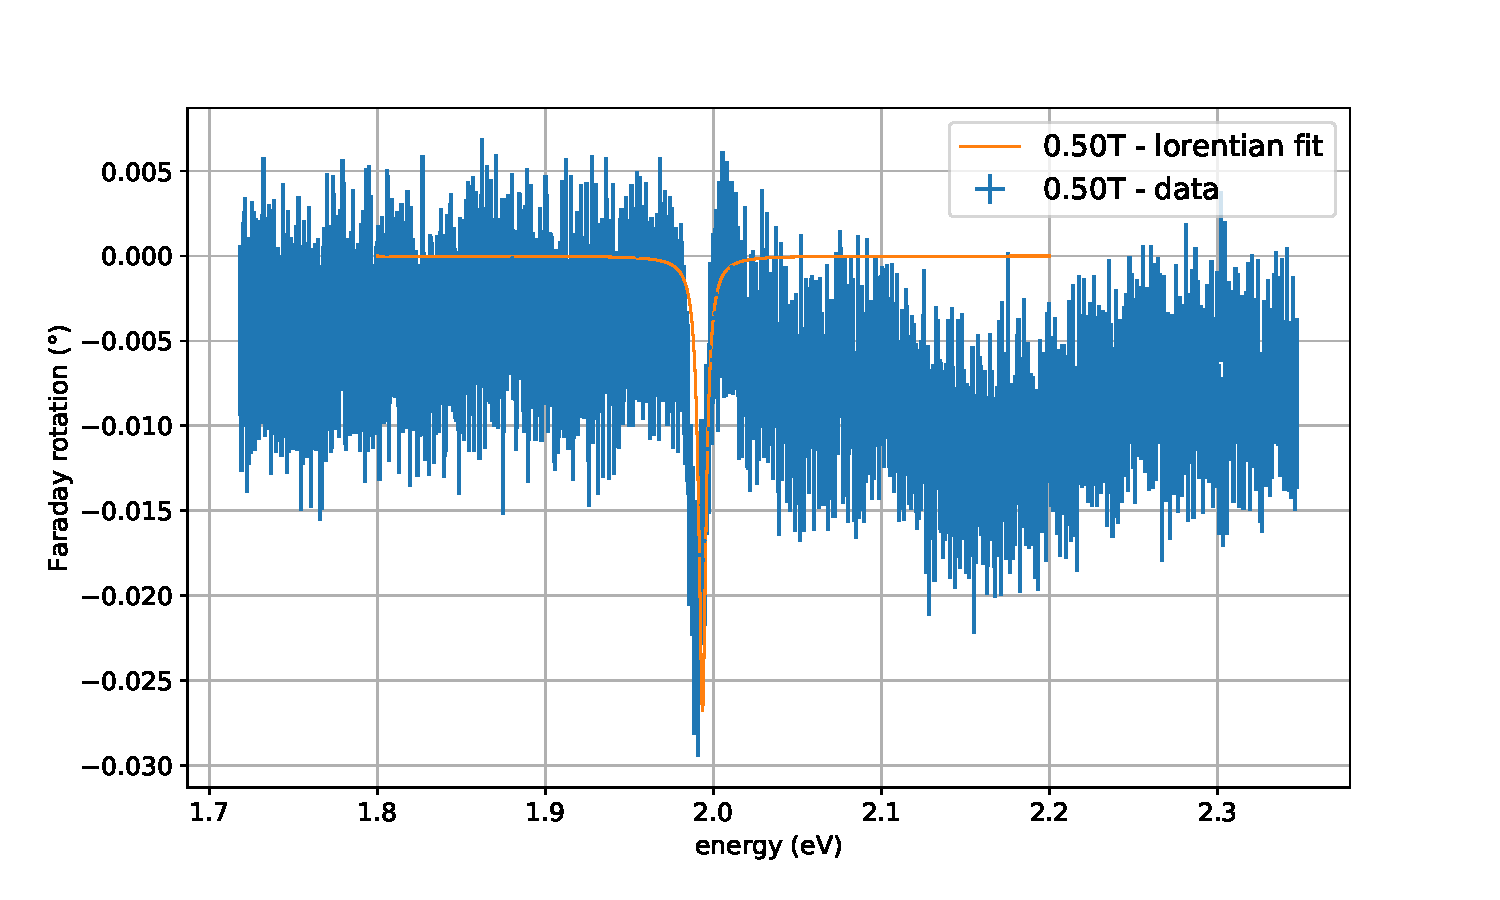
\includegraphics[width=1.0\textwidth]{plots/WS2_500mT.pdf}
    \caption{}
    %label{fig_antibunch_background_comp}
    \end{subfigure}
    %\hfill
    \begin{subfigure}{0.47\textwidth}
        \centering
        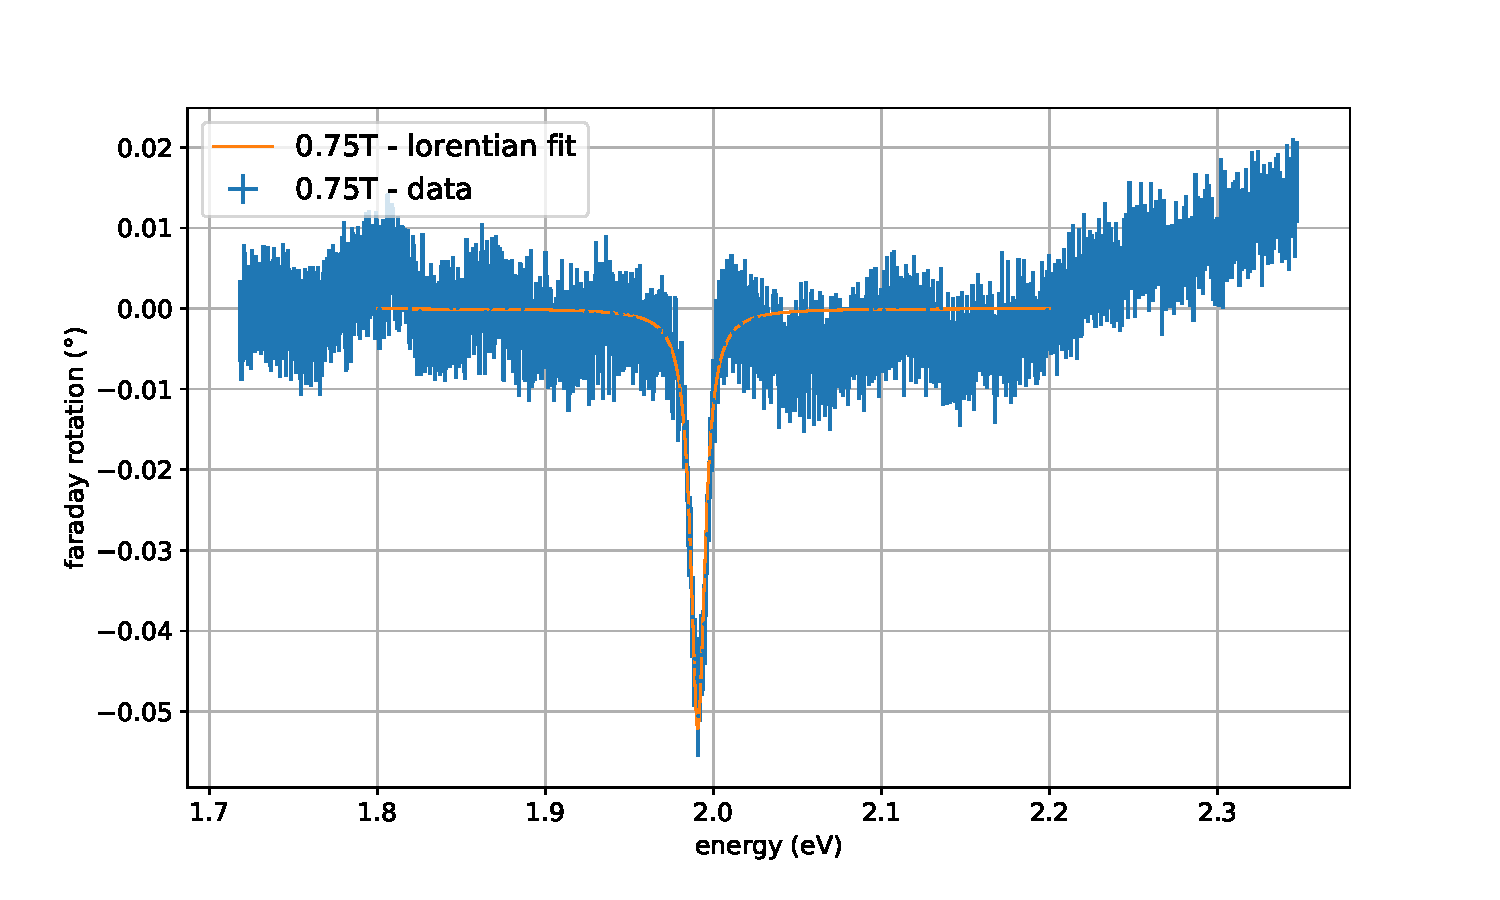
\includegraphics[width=\textwidth]{plots/WS2_750mT.pdf}
        \caption{}
    \end{subfigure}
    \caption{a: Representation of WS$_2$ monolayer data points of the faraday rotation with external magnetic field of \SI{0.50}{\tesla} and lorentian fit. b: Same as a, but at \SI{0.75}{\tesla}.} %hoffe ok, dass der eine so doppelt ist
\end{figure}

\begin{figure}[H]
    \centering
    \begin{subfigure}{0.47\textwidth}
        \centering
        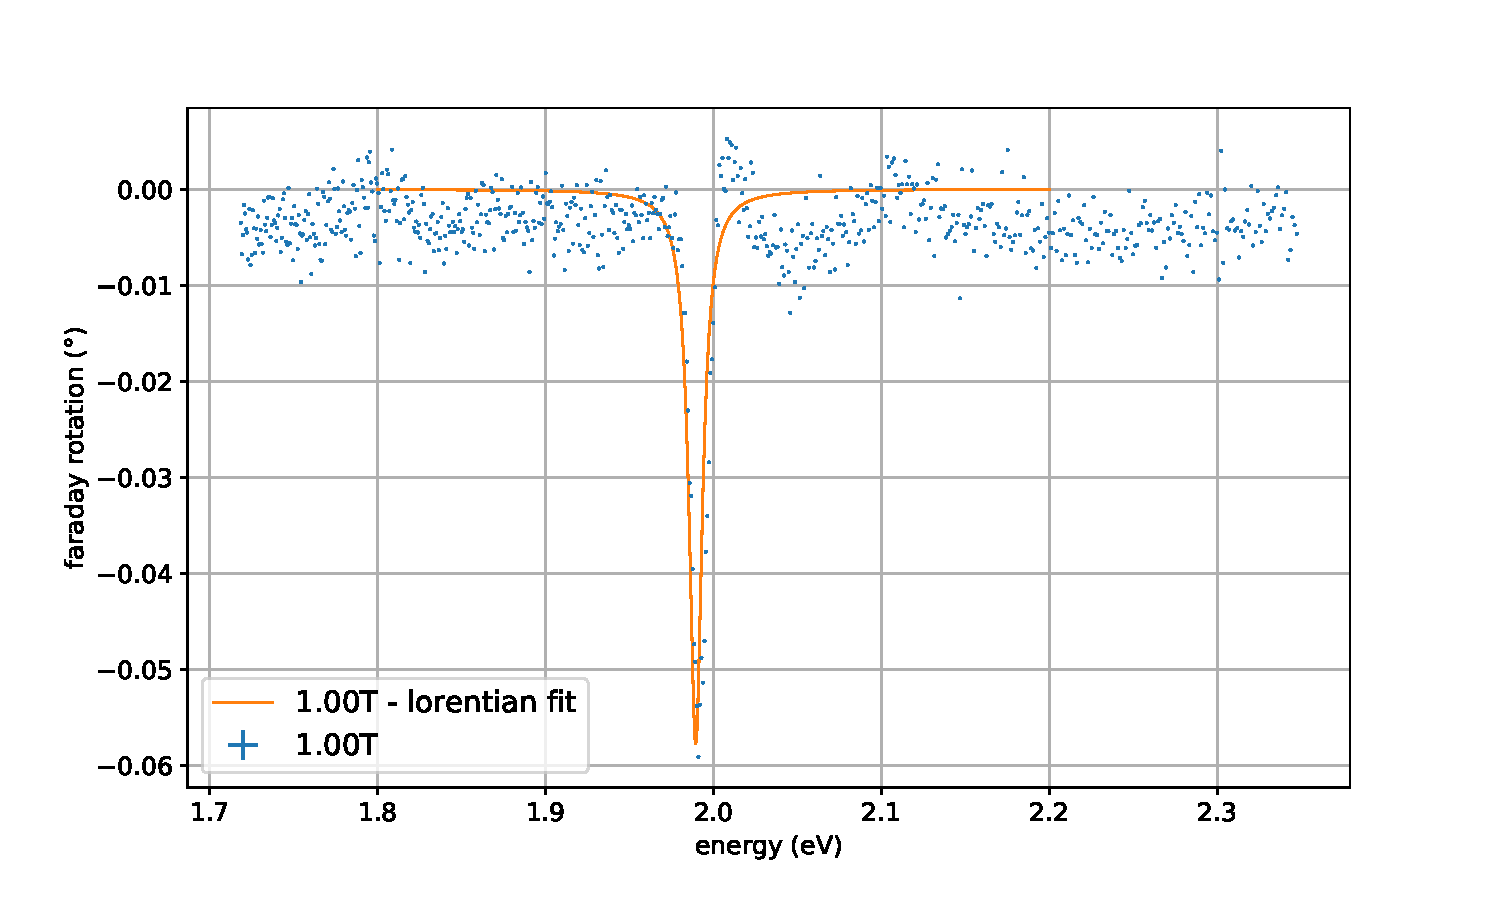
\includegraphics[width=1.0\textwidth]{plots/WS2_1000mT.pdf}
    \caption{}
    %label{fig_antibunch_background_comp}
    \end{subfigure}
    %\hfill
    \begin{subfigure}{0.47\textwidth}
        \centering
        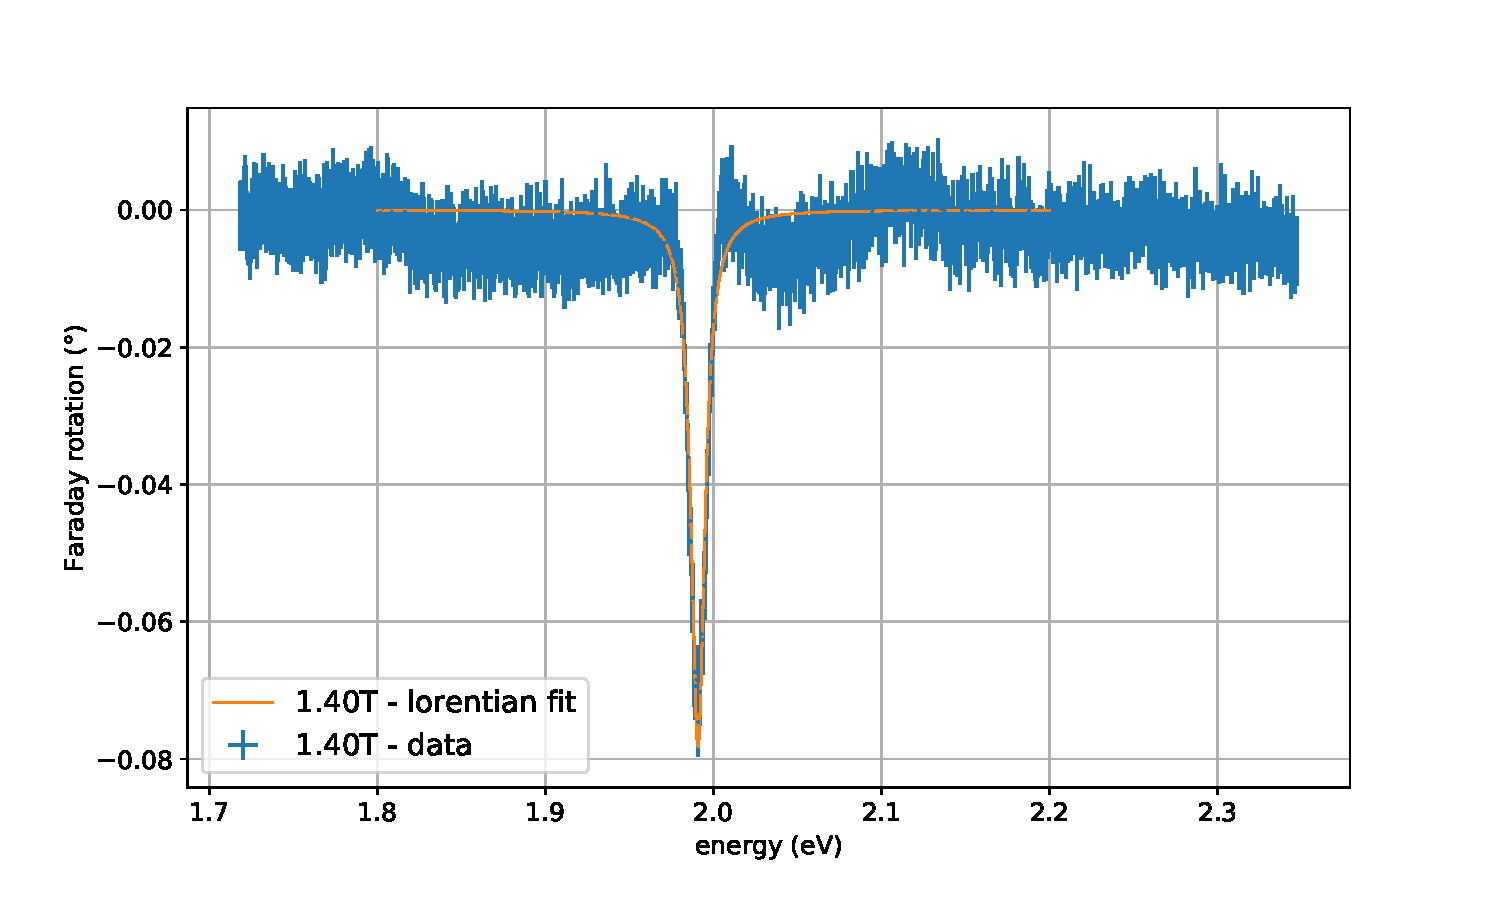
\includegraphics[width=\textwidth]{plots/WS2_1400mT.pdf}
        \caption{}
    \end{subfigure}
    \caption{a: Representation of WS$_2$ monolayer data points of the faraday rotation with external magnetic field of \SI{1.0}{\tesla} and lorentian fit. b: Same as a, but at \SI{1.4}{\tesla}.} %hoffe ok, dass der eine so doppelt ist
\end{figure}

	\printbibliography


\end{document}
